\documentclass[12pt, a4]{report}
    \usepackage[utf8]{inputenc}
    \usepackage[croatian]{babel}
    \usepackage{graphicx}
    \usepackage[a4paper, total={6in, 10in}]{geometry}
    \usepackage{caption}
    \usepackage{amsmath}
    \usepackage{subfig}

    \graphicspath{ {res/} }

    \title{Laboratorijska vježba 1}
    \author{Matija Marić, 0036479678}
    \date{\today}

    \begin{document}
        \begin{titlepage}
            \maketitle
        \end{titlepage}

        \tableofcontents{}

        \chapter{Vježba 2 - Operacije na slici}
        \section{Unarne operacije}
            \begin{enumerate}
                \item Naredba \verb|imagesc| prikazuje sliku isto kao i \verb|image| i \verb|imshow|, ali se vrijednosti piksela skaliraju između maksimalnih i minimalnih vrijednosti.
                    Kod \verb|image| vrijednosti su na intervalu [0, 255], a kod \verb|imshow| na intervalu [0, 1].
                \item
                    \begin{equation}
                        imagesc = \frac{255 * (image - min(image))}{max(image) - min(image)}
                    \end{equation}  
                    \begin{equation}
                        imagesc = \frac{1.0 * (imshow - min(imshow))}{max(imshow) - min(imshow)}
                    \end{equation}
                \item
                    \begin{minipage}{\linewidth}
                        \centering
                        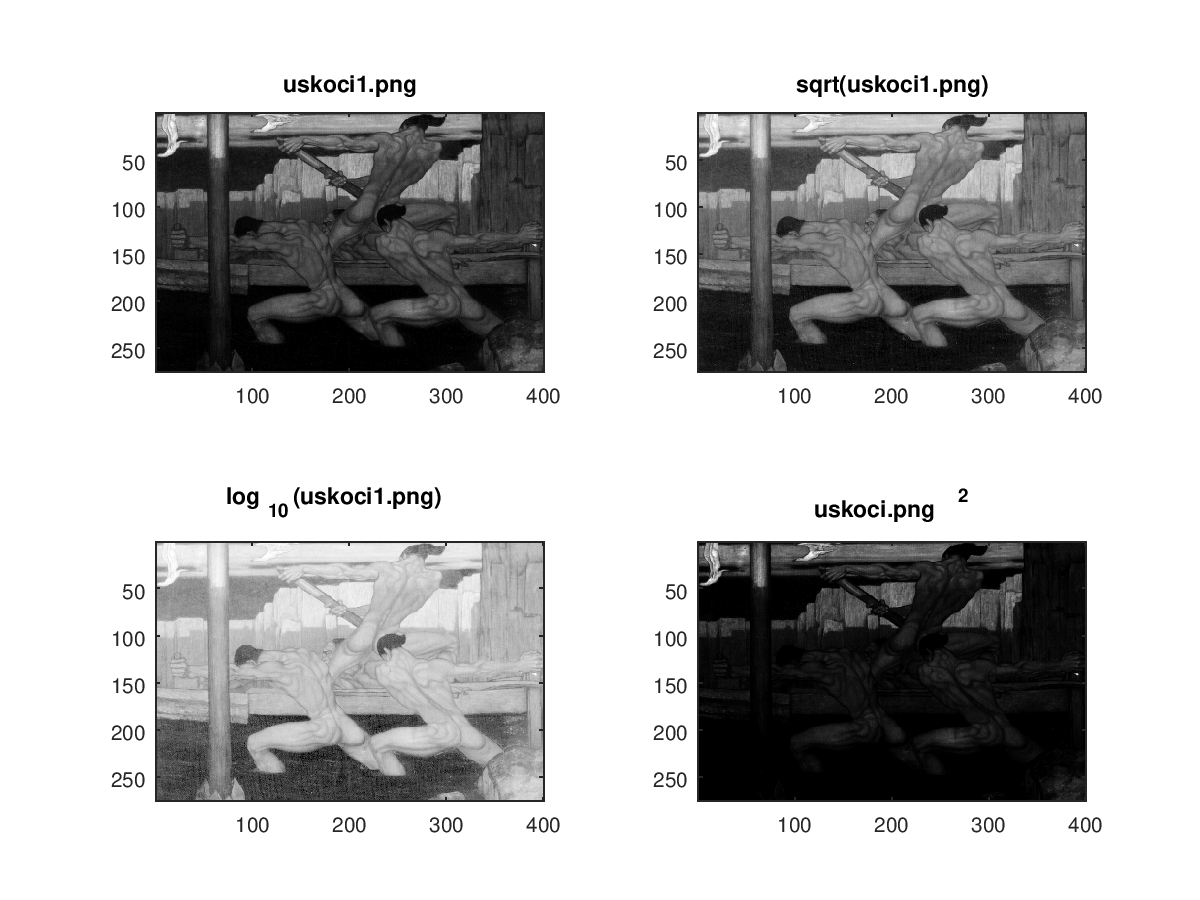
\includegraphics[width=0.75\textwidth]{unary}
                        \captionof{figure}{Unarne operacije}
                    \end{minipage}
                \item
                    \begin{equation}
                        H_1 = N \circ U_1 = N(log x)
                    \end{equation}
                    \begin{equation}
                        H_2 = N \circ U_2 = N(\sqrt x)
                    \end{equation}
                    \begin{equation}
                        H_3 = N \circ U_3 = N(x^2)
                    \end{equation}
                \item
                    \begin{minipage}{\linewidth}
                        \centering
                        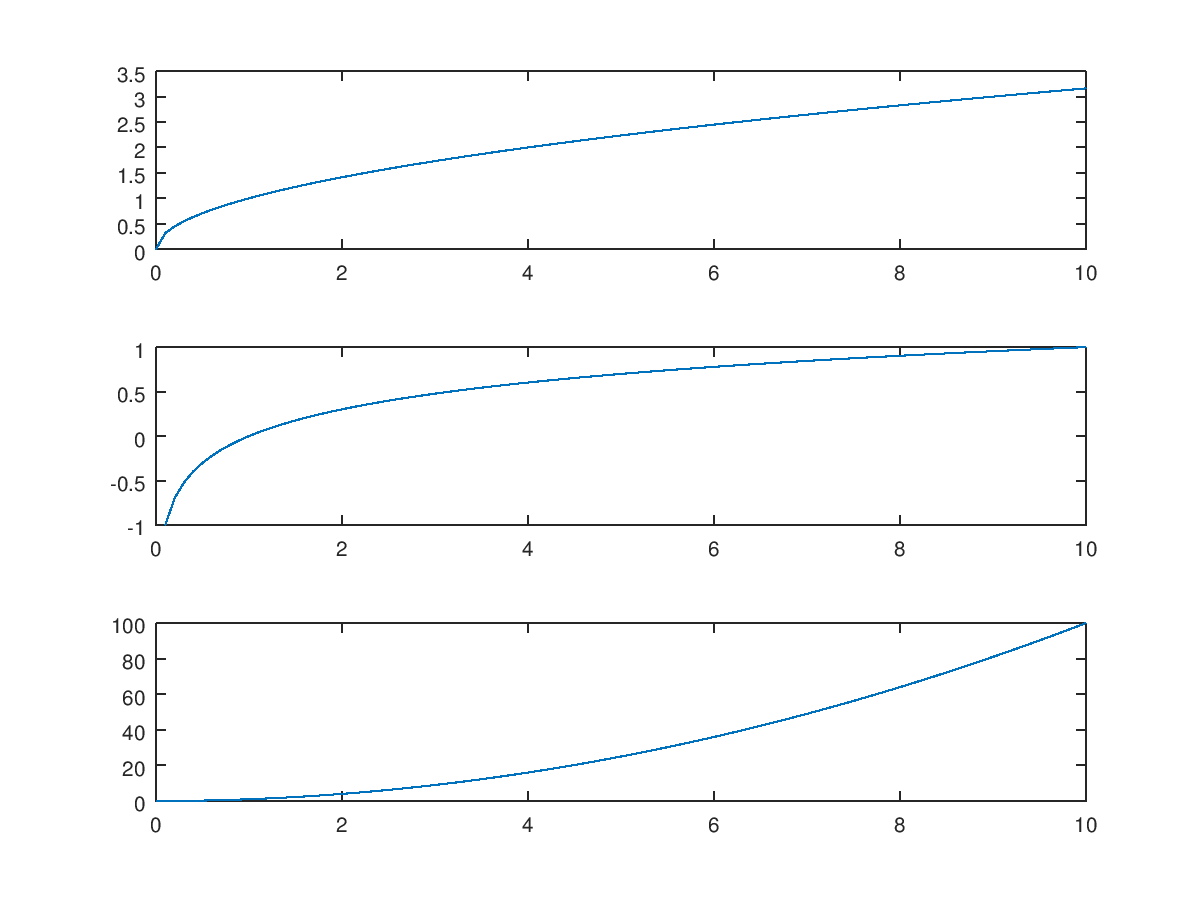
\includegraphics[width=0.75\textwidth]{transfer}
                        \captionof{figure}{Prijenosne funkcije}
                    \end{minipage}
            \end{enumerate}
        \section{Binarne operacije}
            \begin{enumerate}
                \item
                    \begin{minipage}{\linewidth}
                        \centering
                        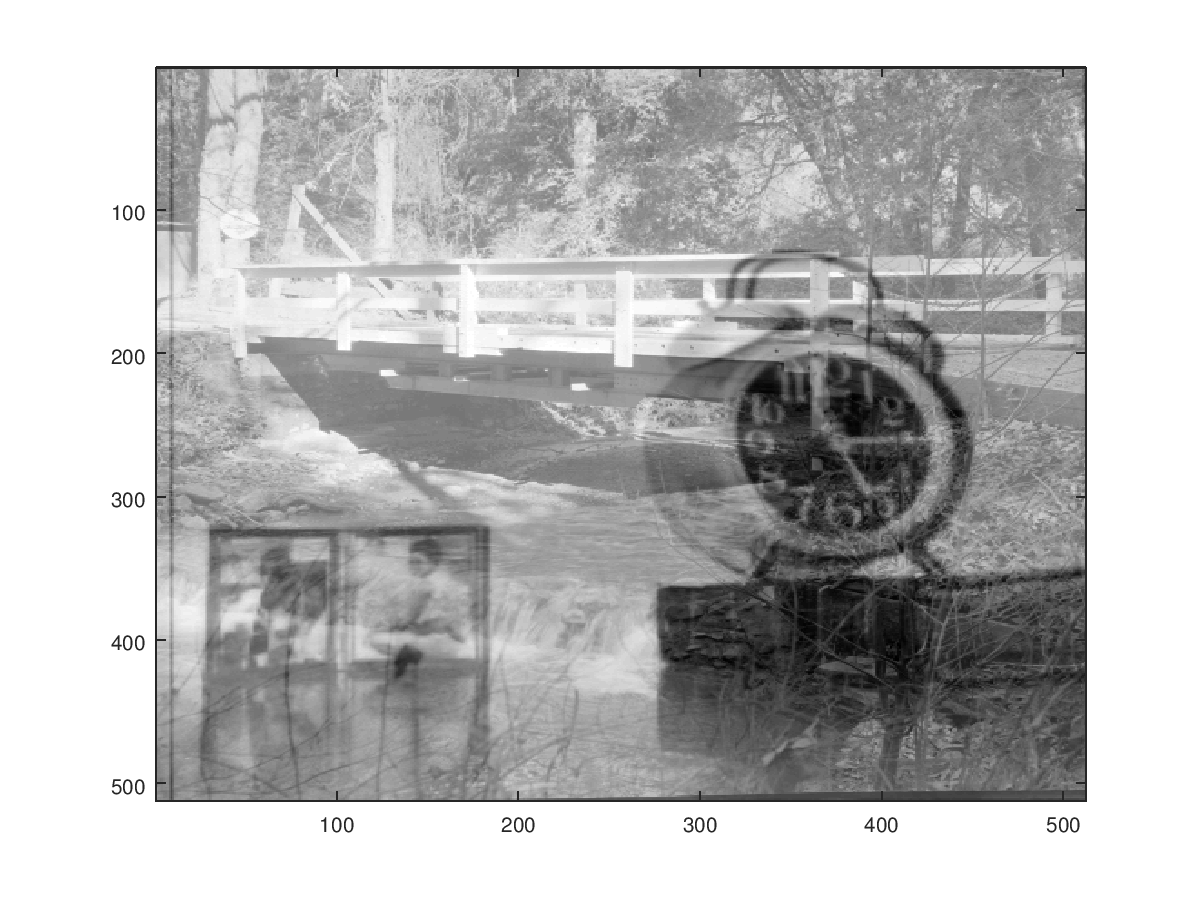
\includegraphics[width=0.75\textwidth]{binarysum}
                        \captionof{figure}{Zbroj dvije crno-bijele slike}
                    \end{minipage}
                    \begin{minipage}{\linewidth}
                        \centering
                        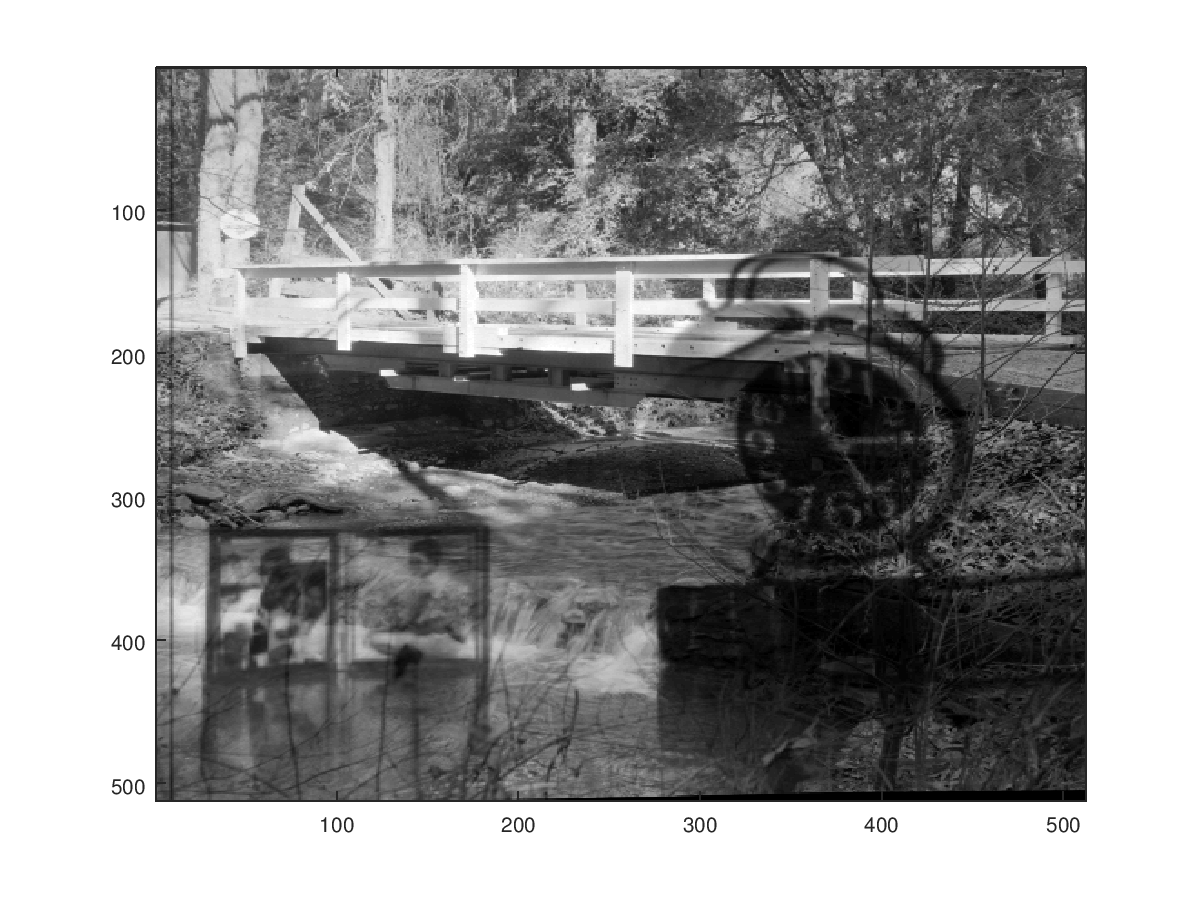
\includegraphics[width=0.75\textwidth]{binarymul}
                        \captionof{figure}{Umnožak dvije crno-bijele slike}
                    \end{minipage}
                    \begin{minipage}{\linewidth}
                        \centering
                        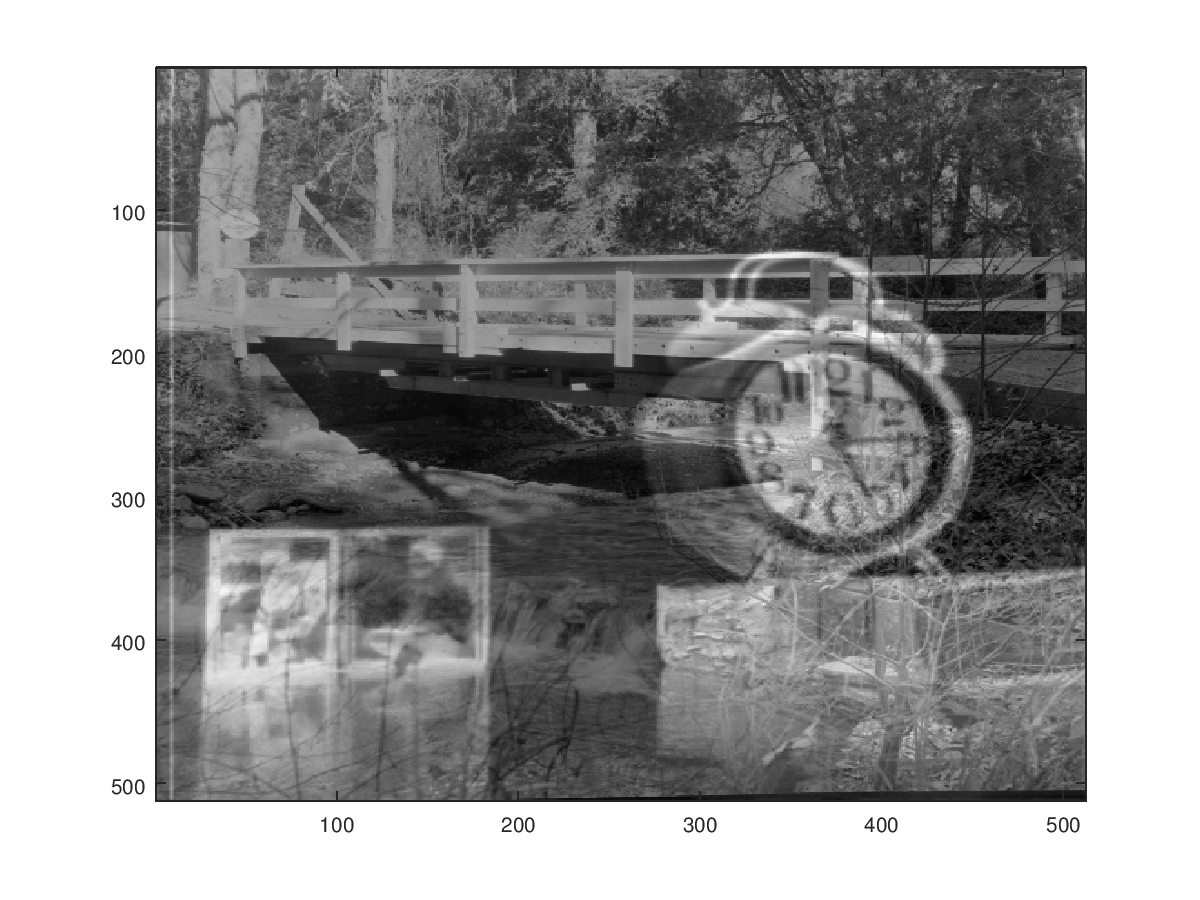
\includegraphics[width=0.75\textwidth]{binarysub}
                        \captionof{figure}{Razlika dvije crno-bijele slike}
                    \end{minipage}
                \item
                    \begin{minipage}{\linewidth}
                        \centering
                        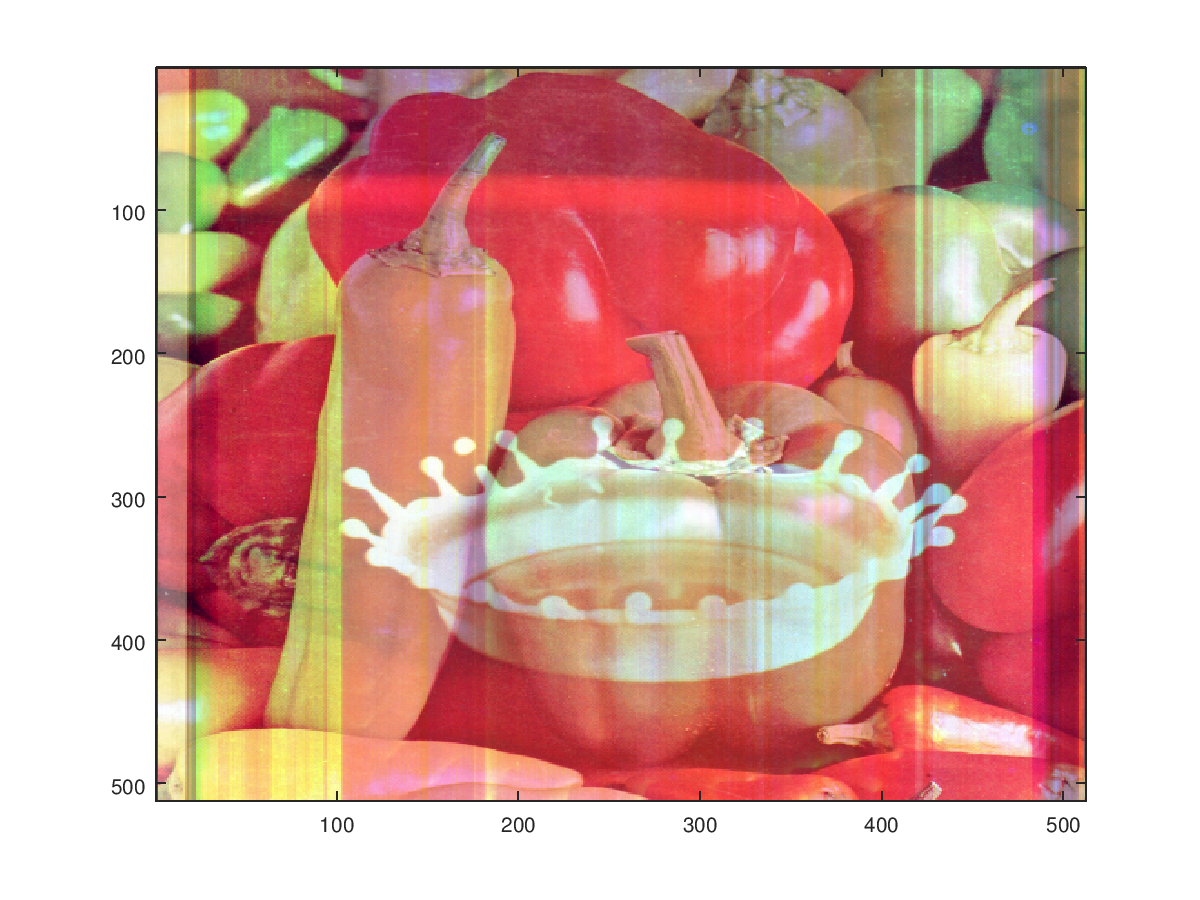
\includegraphics[width=0.75\textwidth]{binarysumrgb}
                        \captionof{figure}{Zbroj dvije slike u boji}
                    \end{minipage}
                    \begin{minipage}{\linewidth}
                        \centering
                        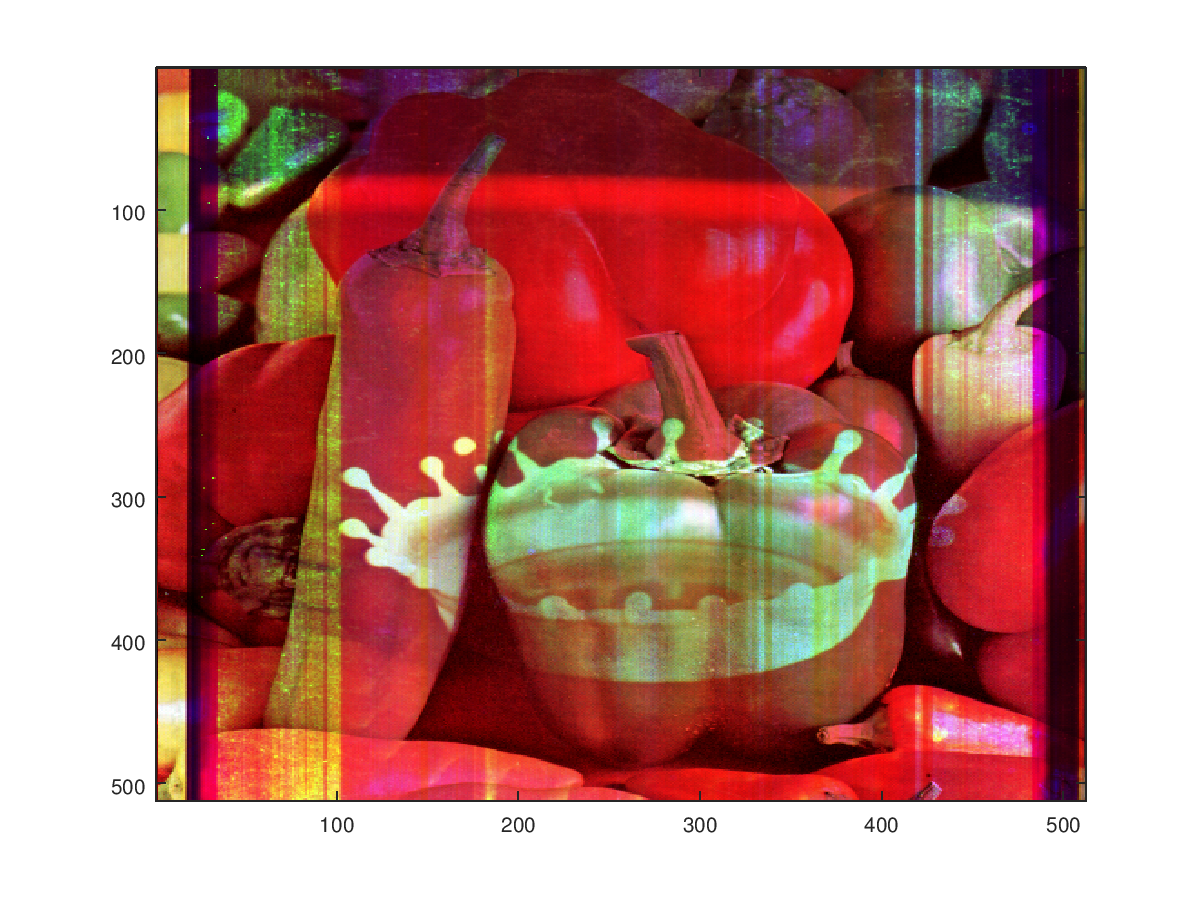
\includegraphics[width=0.75\textwidth]{binarymulrgb}
                        \captionof{figure}{Umnožak dvije slike u boji}
                    \end{minipage}
                    \begin{minipage}{\linewidth}
                        \centering
                        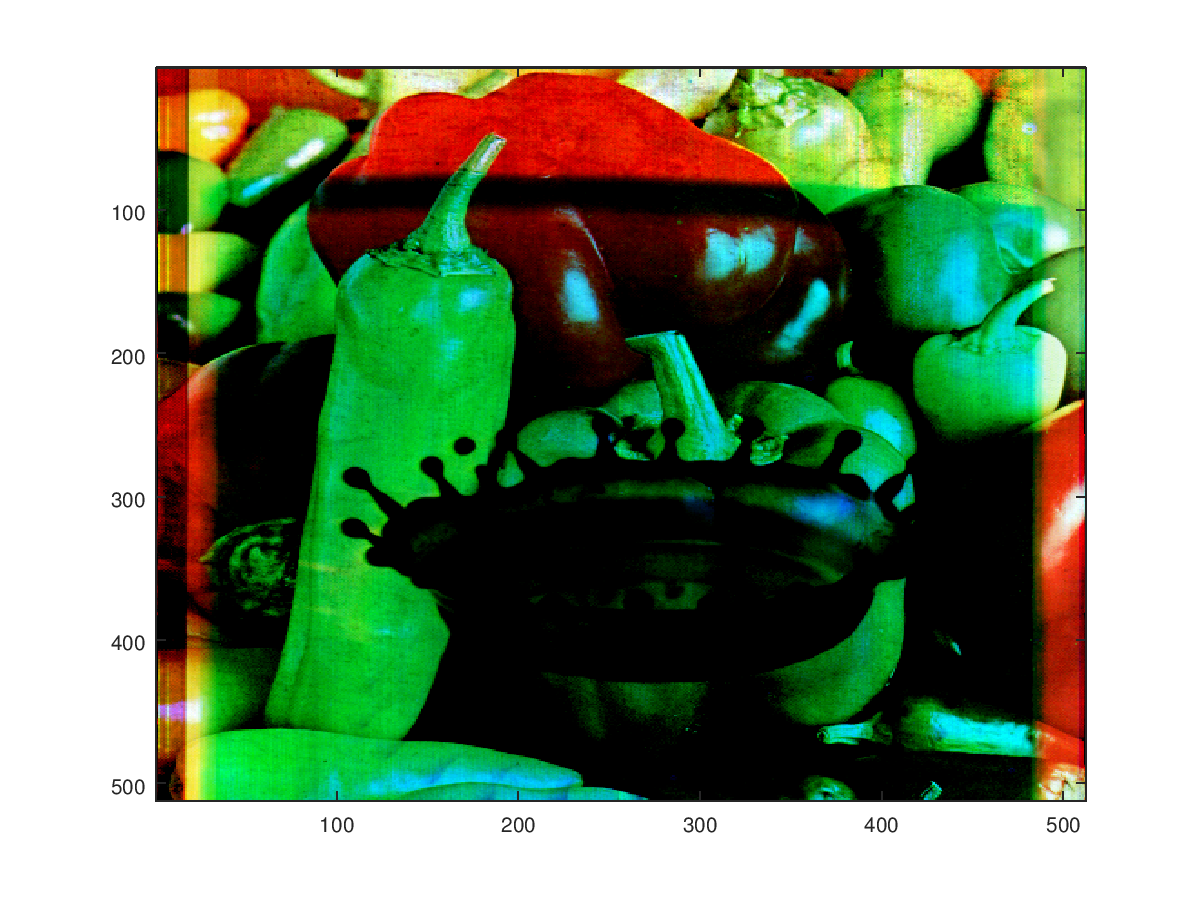
\includegraphics[width=0.75\textwidth]{binarysubrgb}
                        \captionof{figure}{Razlika dvije slike u boji}
                    \end{minipage}
            \end{enumerate}
        \section{Digitalna angiografija}
            \begin{minipage}{\linewidth}
                \centering
                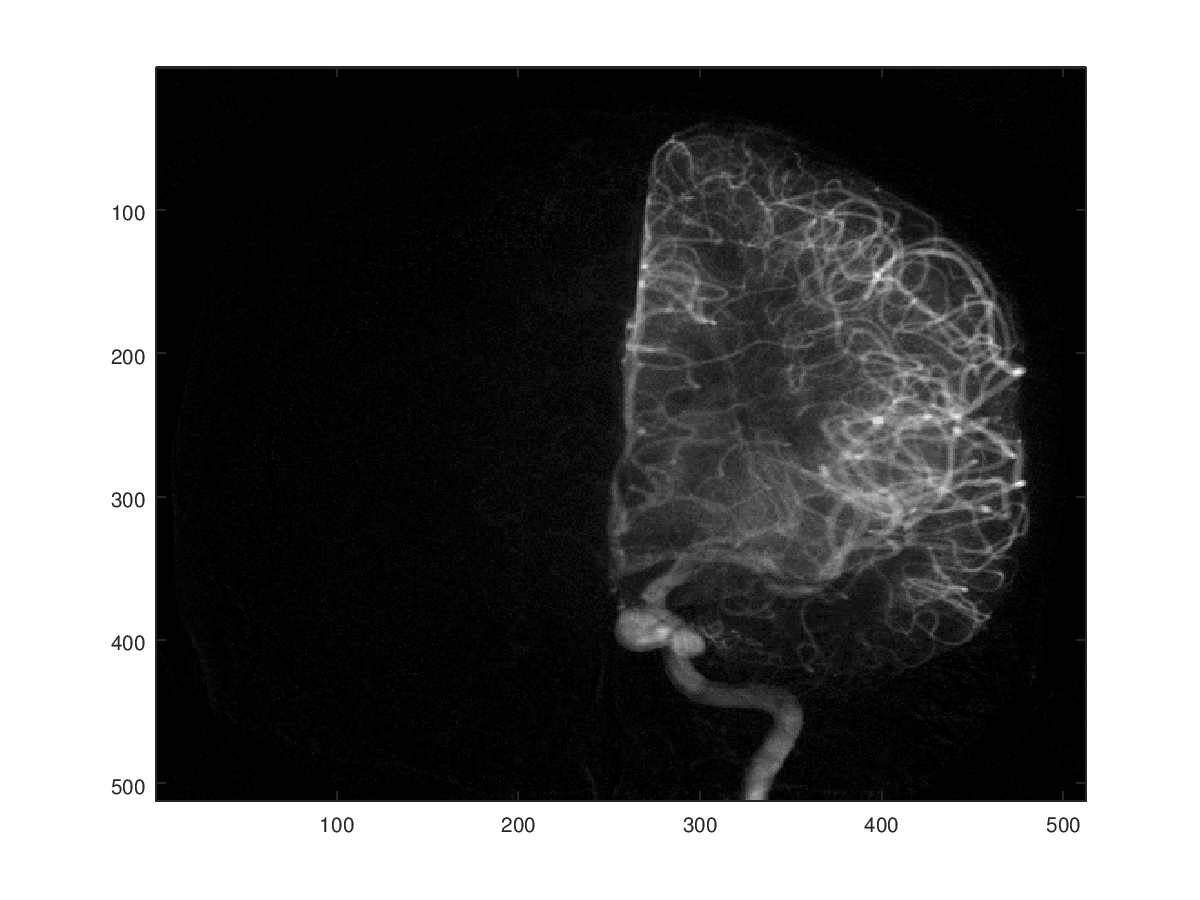
\includegraphics[width=0.75\textwidth]{angio}
                \captionof{figure}{Razlika angiografskih snimki sa i bez kontrasta}
            \end{minipage}
        \section{Gama korekcija}
            \begin{enumerate}
                \item
                    \begin{minipage}{\linewidth}
                        \centering
                        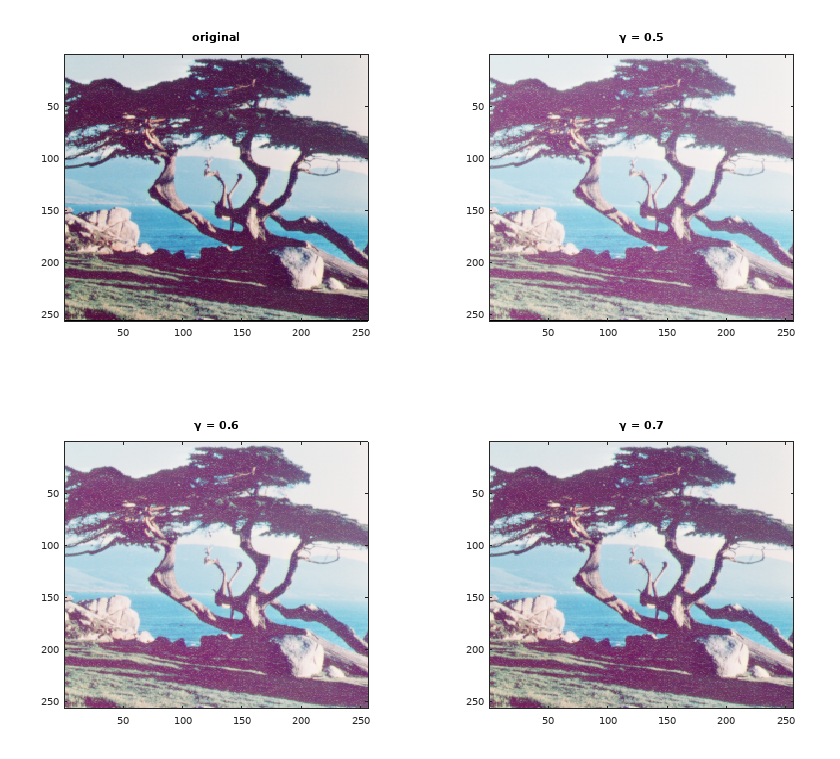
\includegraphics[width=0.75\textwidth]{gamma}
                        \captionof{figure}{Gama korekcija sa različitim vrijednostima $\gamma$}
                    \end{minipage}
                \item
                    Vrijednosti $\gamma$ kojima sam kalibrirao za svoj ekran su:
                    \begin{equation}
                        \vec \gamma = \left< 4, 4, 4 \right>
                    \end{equation}
                    \begin{minipage}{\linewidth}
                        \centering
                        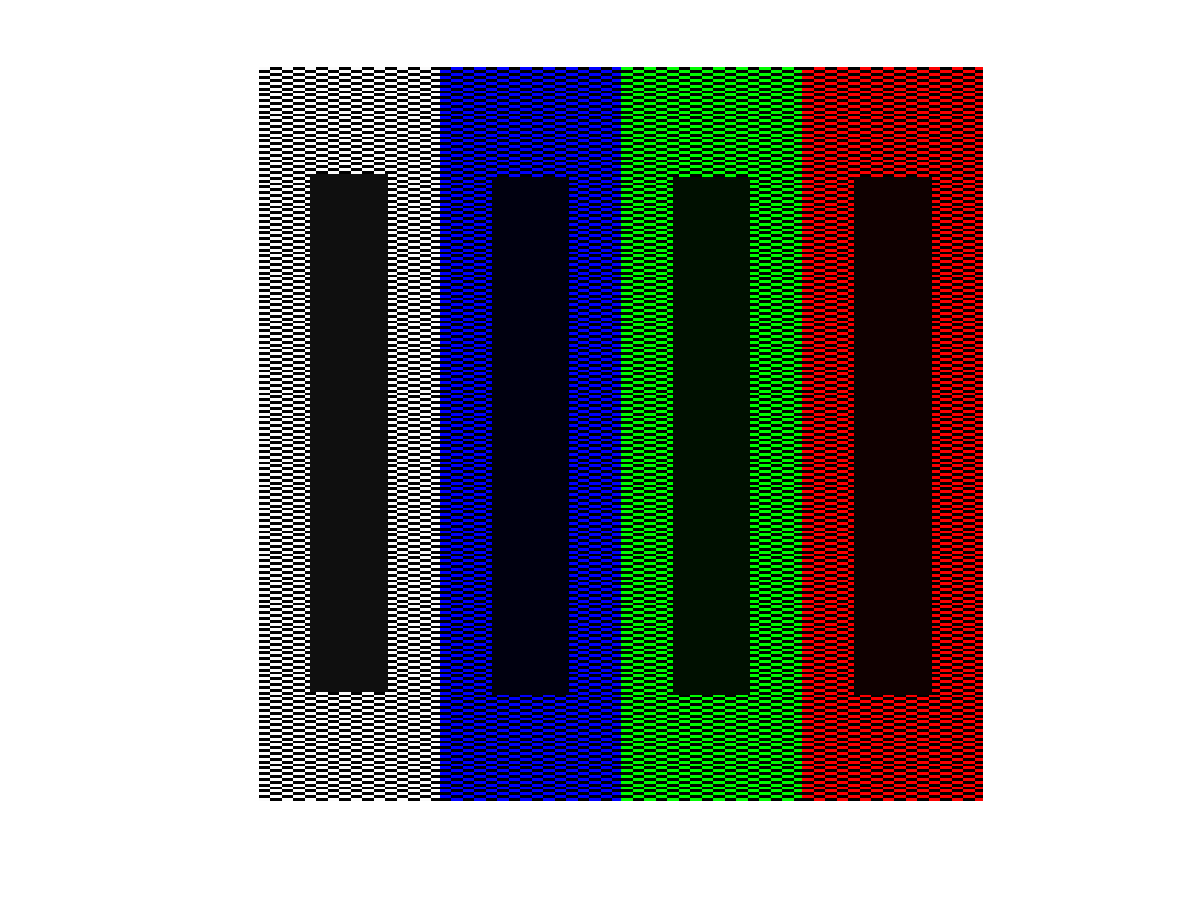
\includegraphics[width=0.75\textwidth]{gamma_correction}
                        \captionof{figure}{Slika za kalibraciju gama korekcije na monitoru}
                    \end{minipage}
                \item
                    Gama korekcija je unarna operacija je se radi na jednoj slici.
            \end{enumerate}
        \section{Linearna konvolucija}
            \begin{enumerate}
                \item
                    \begin{minipage}{\linewidth}
                        \centering
                        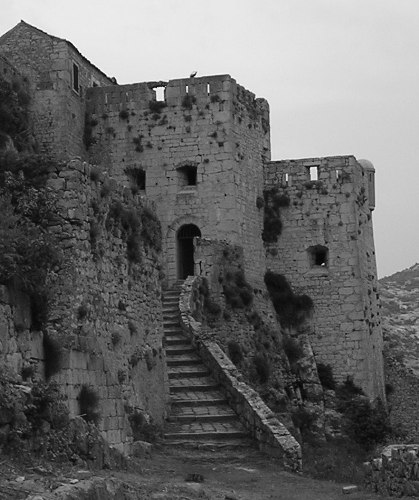
\includegraphics[width=0.4\textwidth]{klis2}
                        \captionof{figure}{Originalna slika na kojoj radimo konvoluciju}
                    \end{minipage}
                    \begin{minipage}{\linewidth}
                        \centering
                        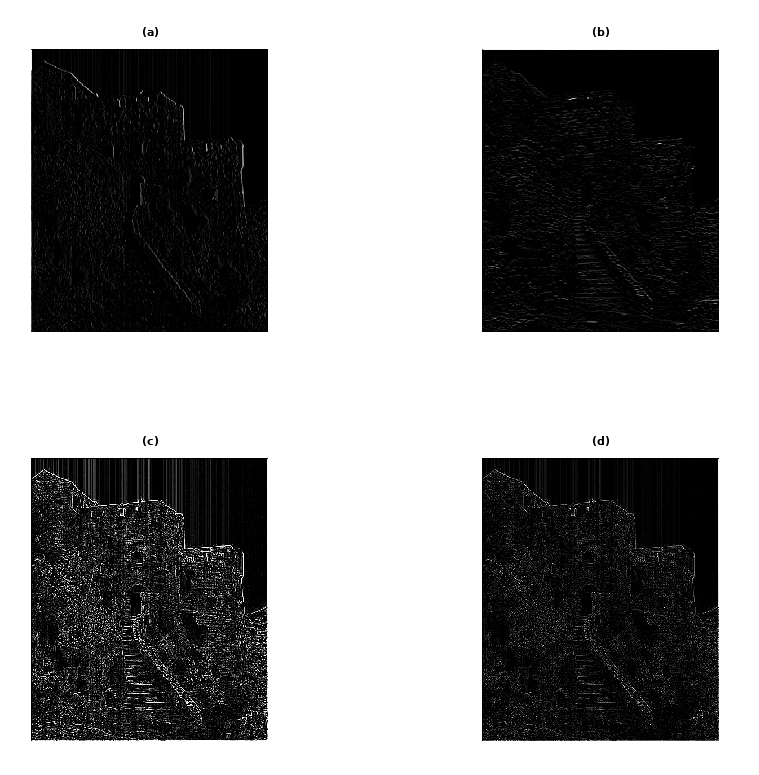
\includegraphics[width=0.75\textwidth]{conv2d}
                        \captionof{figure}{Konvolucija slike sa različitim konvolucijskim maskama}
                    \end{minipage}\\
                    Korištene maske su:
                    \begin{equation}
                        \frac{1}{4}
                        \begin{bmatrix}
                            1 & 0 & -1 \\
                            2 & 0 & -2 \\
                            1 & 0 & -1
                        \end{bmatrix},
                        \frac{1}{3}
                        \begin{bmatrix}
                            1 & 1 & 1 \\
                            0 & 0 & 0 \\
                            -1 & -1 & -1
                        \end{bmatrix},
                        \begin{bmatrix}
                            -1 & -1 & -1 \\
                            -1 & 8 & -1 \\
                            -1 & -1 & -1
                        \end{bmatrix},
                        \begin{bmatrix}
                            0 & -1 & 0 \\
                            -1 & 4 & -1 \\
                            0 & -1 & 0
                        \end{bmatrix}
                    \end{equation}
                \item
                    Odzivi na maske (a) i (b) daju vertikalne i horizontalne rubove na slici, a (c) i (d) daju sve rubove.
                \item
                    \begin{minipage}{\linewidth}
                        \centering
                        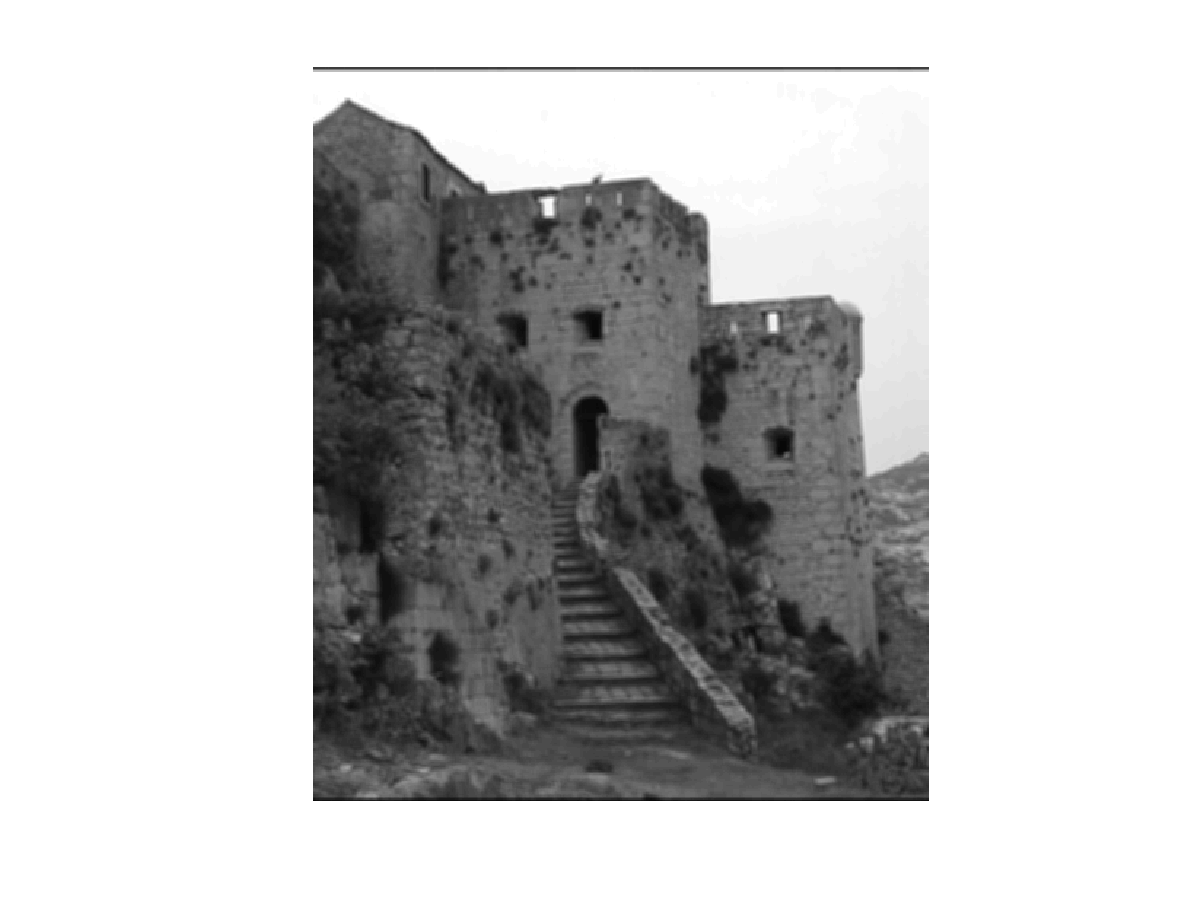
\includegraphics[width=0.75\textwidth]{convAvg}
                        \captionof{figure}{Slika sa konvolucijskom maskom za usrednjavanje}
                    \end{minipage}
                \item
                    Korištena je maska:
                    \begin{equation}
                        \begin{bmatrix}
                            1 & 1 & 1 & 1 \\
                            1 & 1 & 1 & 1 \\
                            1 & 1 & 1 & 1 \\
                            1 & 1 & 1 & 1
                        \end{bmatrix}
                    \end{equation}
                \item
                    Bila je potrebna normalizacija slike jer je konvolucija sumiranje za svaki element matrice maskiranja. Vrijednost svakog piksela se uveća i do 16 puta za masku 4x4.
                \item
                    Konvolucija je binarna operacija jer je jedan operator slika, a drugi konvolucijska maska.
            \end{enumerate}
        \chapter{Vježba 3 - Otipkavanje i kvantizacija}
        \section{Kvantizacija}
            \begin{enumerate}
                \item 
                    Funkcija \verb|quant(x, d)| vraća vrijednosti \verb|x| zaokružene na najbliži višekratnik \verb|d|.  
                \item
                    Kako bi kvantizirali signal u točno N razina koristimo sljedeći izraz:
                    \begin{equation}
                        quant\_N(x, N) = quant(x, \frac{max(x) - min(x)}{N - 1})
                    \end{equation}
                \item
                    \begin{minipage}{\linewidth}
                        \centering
                        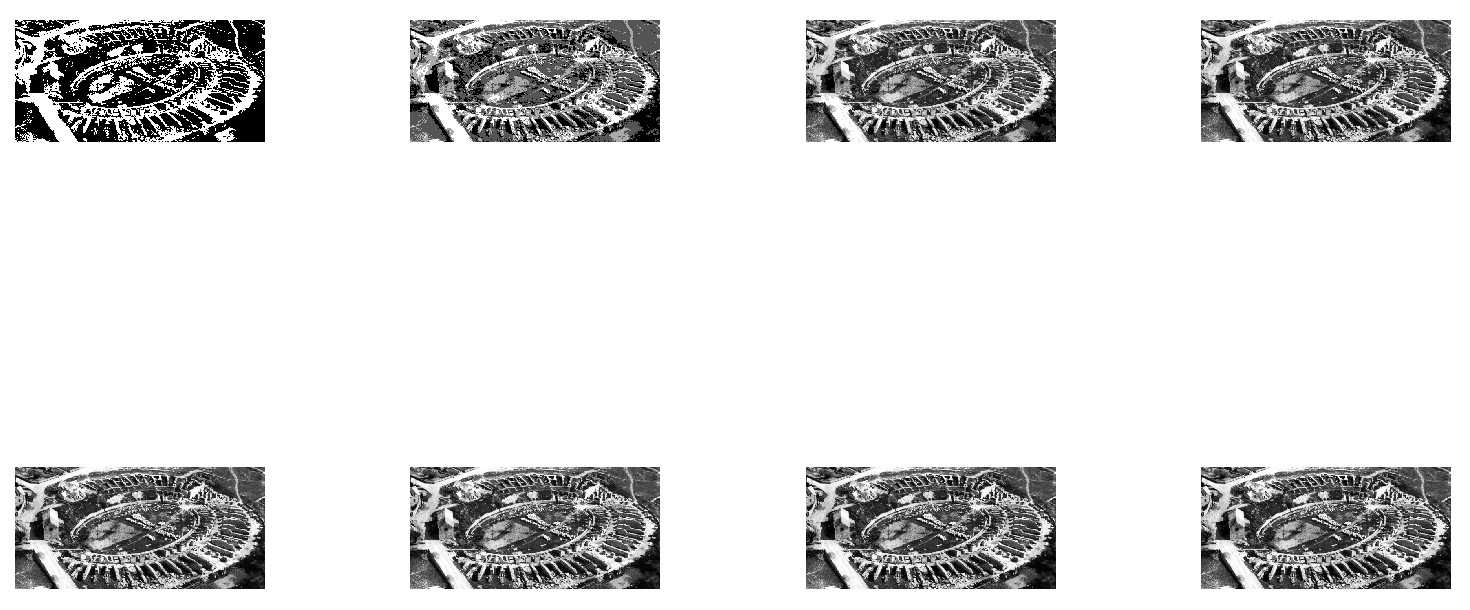
\includegraphics[width=0.75\textwidth]{quant}
                        \captionof{figure}{Slika kvantizirana na N $\in$ [$2^1$,...,$2^8$] razina}
                    \end{minipage}
                \item
                    Razlika se počinje pojavljivati tek ispod 4-5 bitova.
                \item
                    Kvantizacijom na 1 bit svi su pikseli ili crni ili bijeli.
                \item
                    Kvantizacijski šum nastaje zbog zaokruživanja na najbliži višekratnik razine kvantizacije. Najviša vrijednost šuma je pola vrijednosti razine.        
            \end{enumerate}
        \section{Otipkavanje}
            \begin{enumerate}
                \begin{figure}[ht]
                    \centering
                    \begin{tabular}{cc}
                        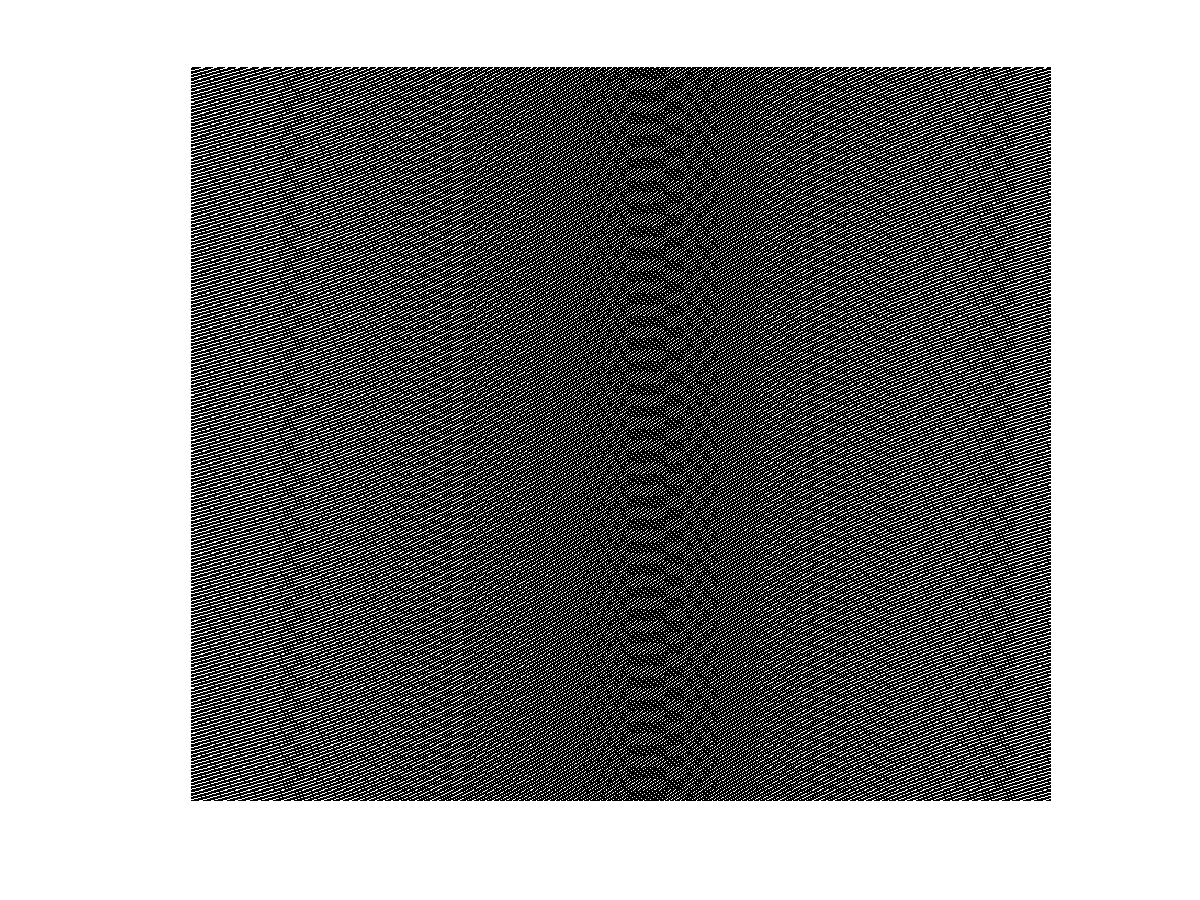
\includegraphics[width=0.35\textwidth]{sample_1} & 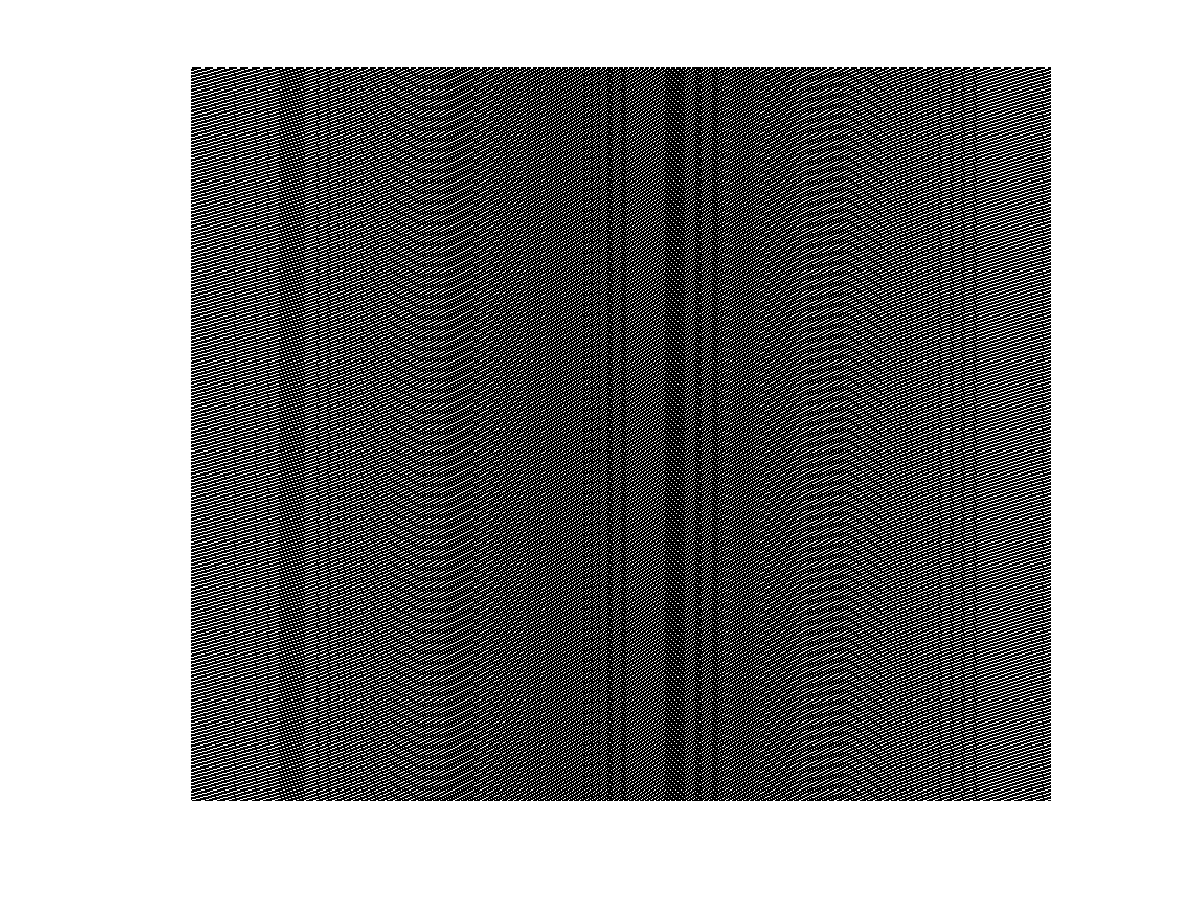
\includegraphics[width=0.35\textwidth]{sample_2} \\
                        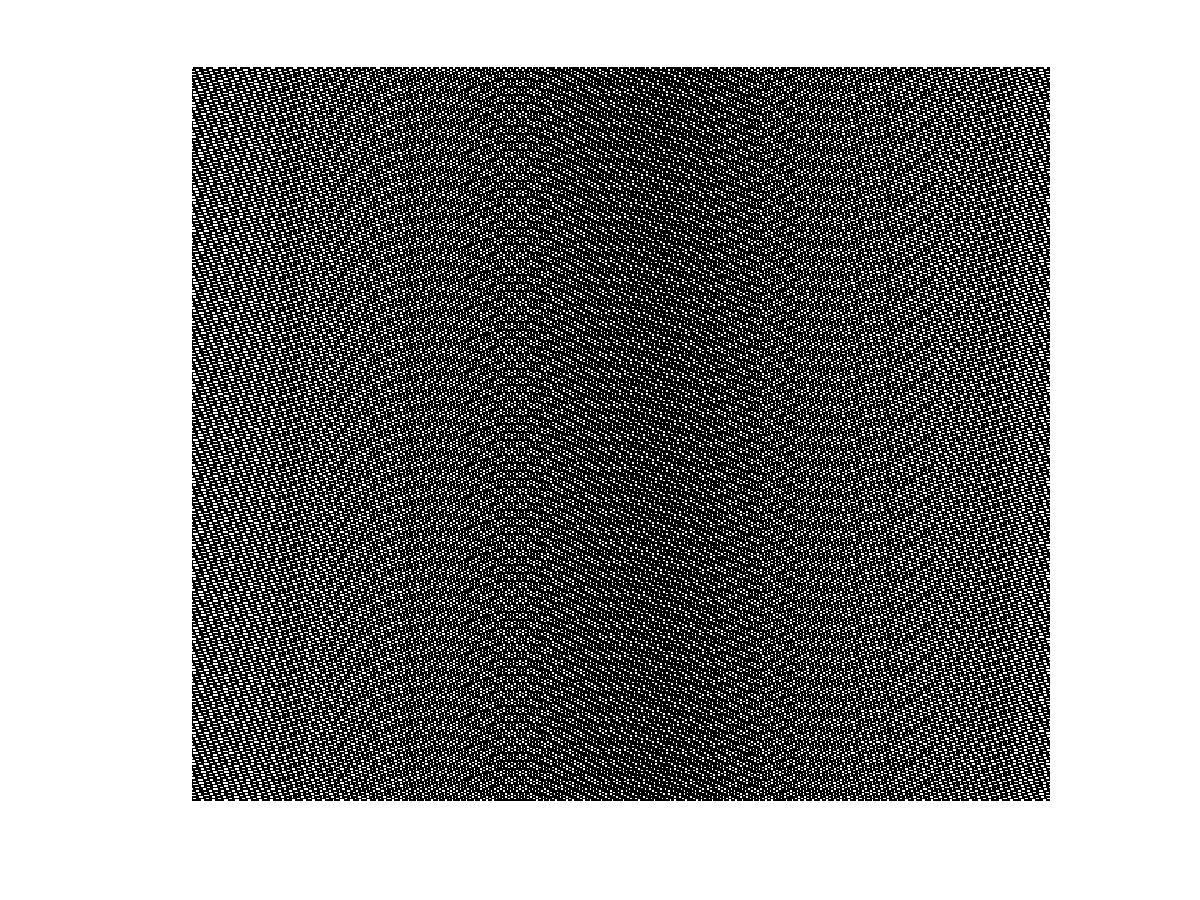
\includegraphics[width=0.35\textwidth]{sample_3} & 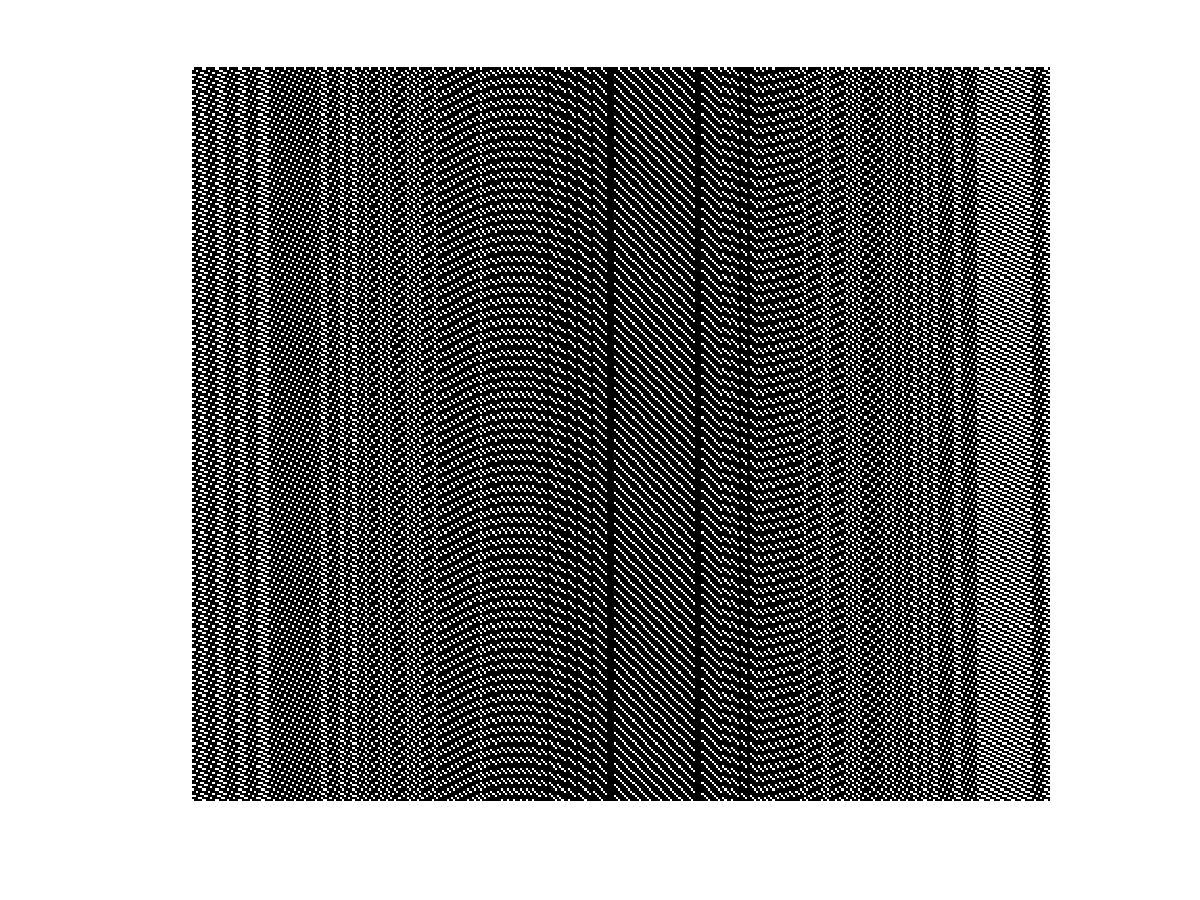
\includegraphics[width=0.35\textwidth]{sample_4} \\
                        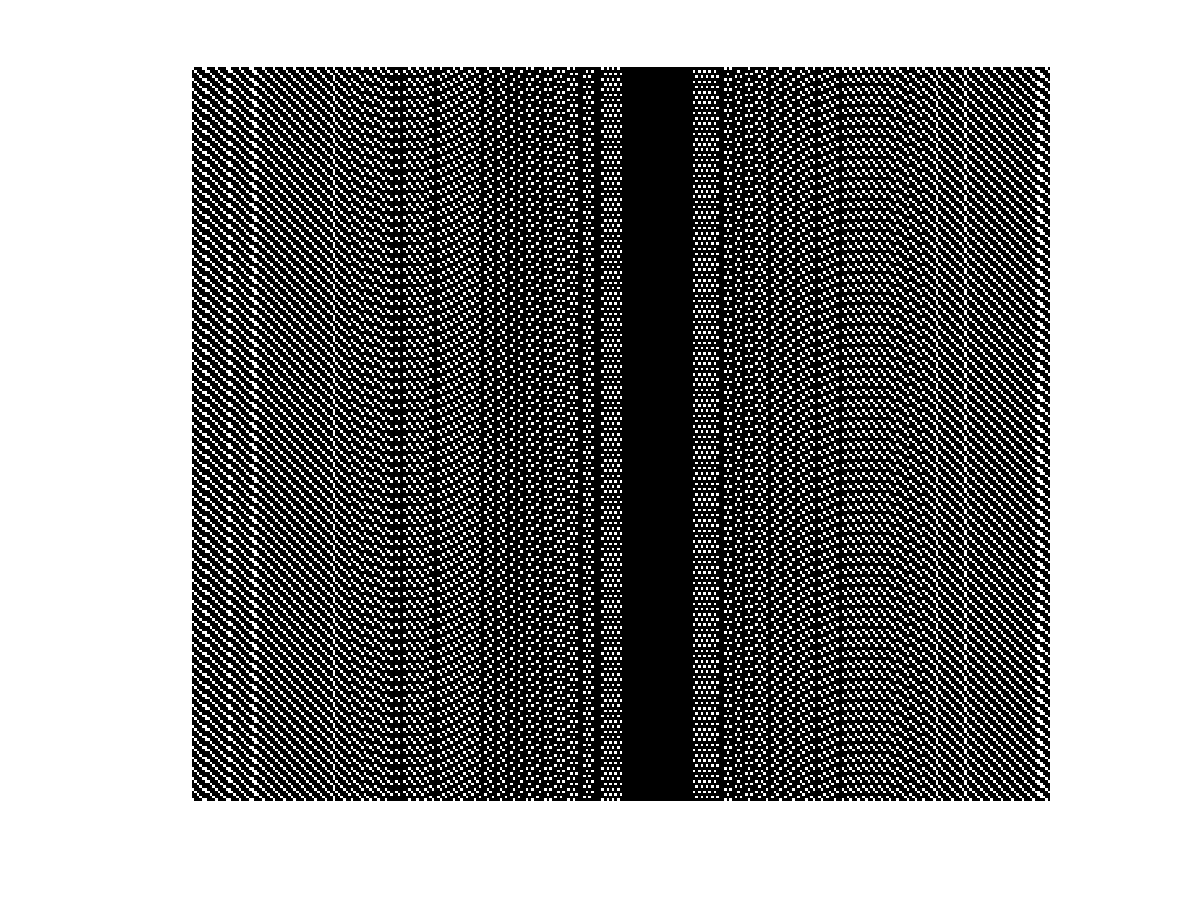
\includegraphics[width=0.35\textwidth]{sample_5} & 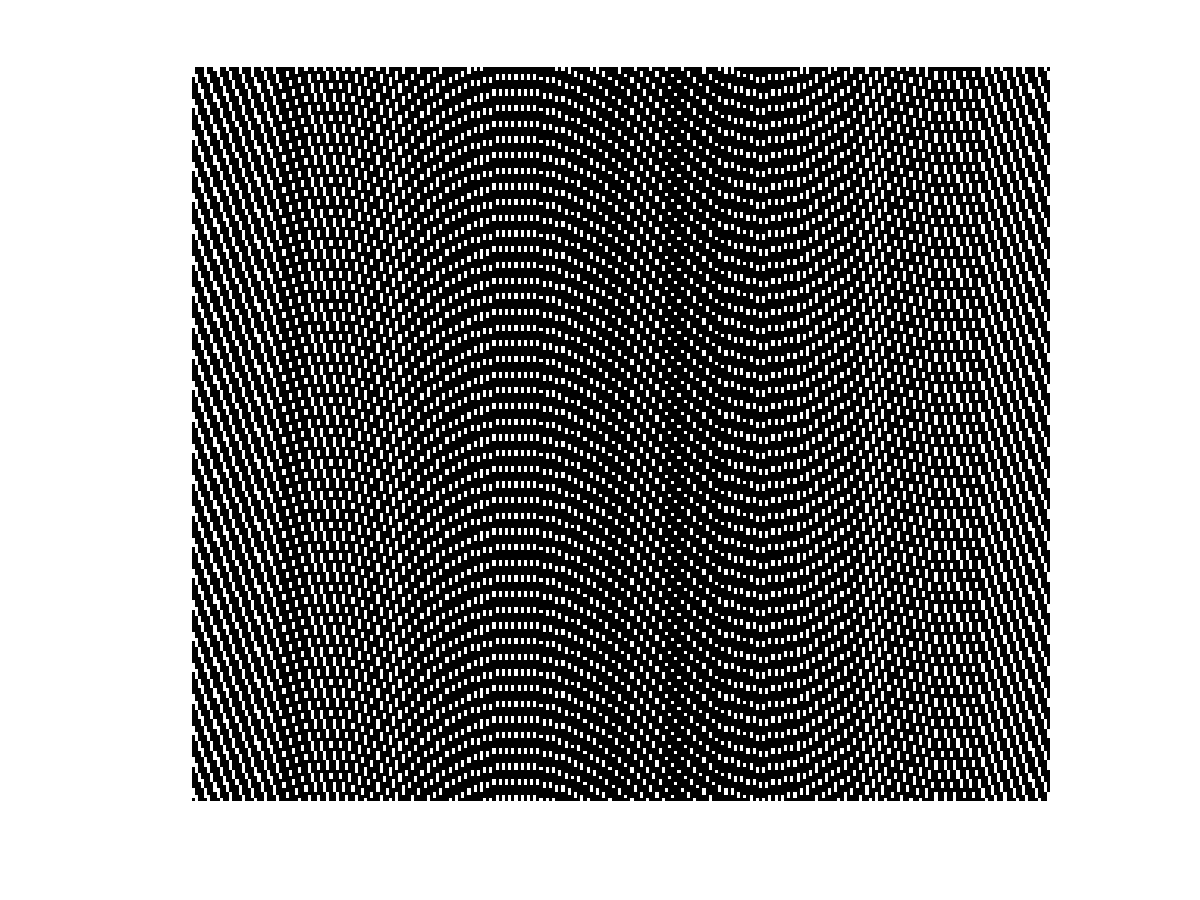
\includegraphics[width=0.35\textwidth]{sample_6} \\
                        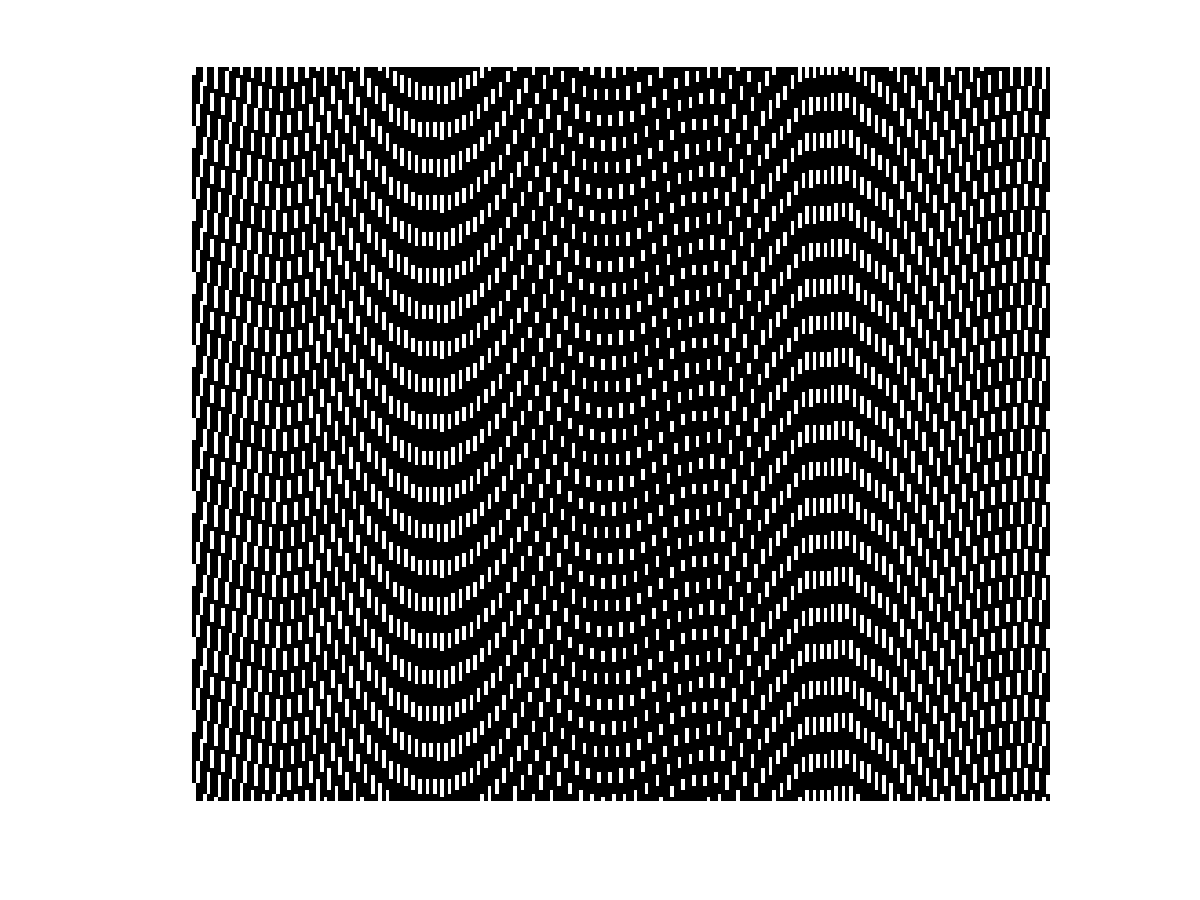
\includegraphics[width=0.35\textwidth]{sample_7} & 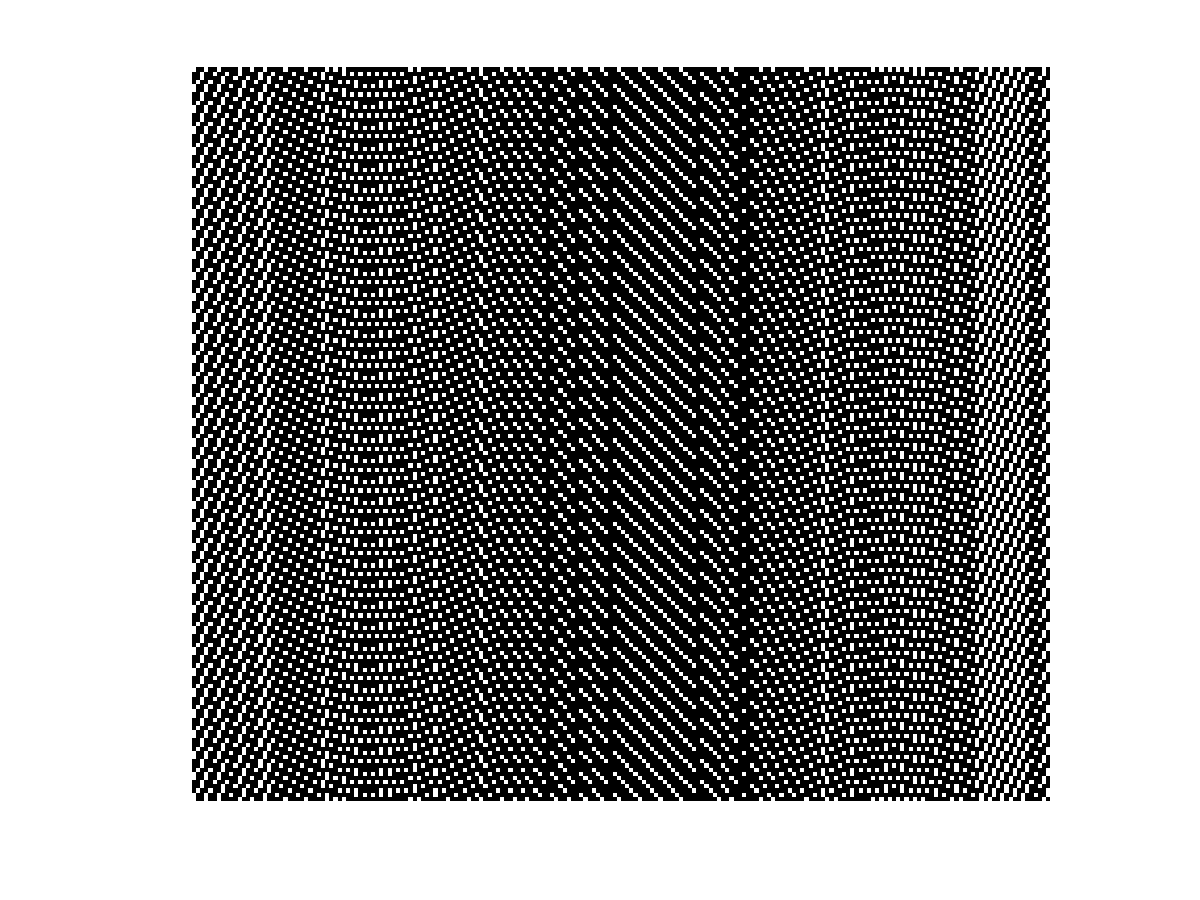
\includegraphics[width=0.35\textwidth]{sample_8} \\
                        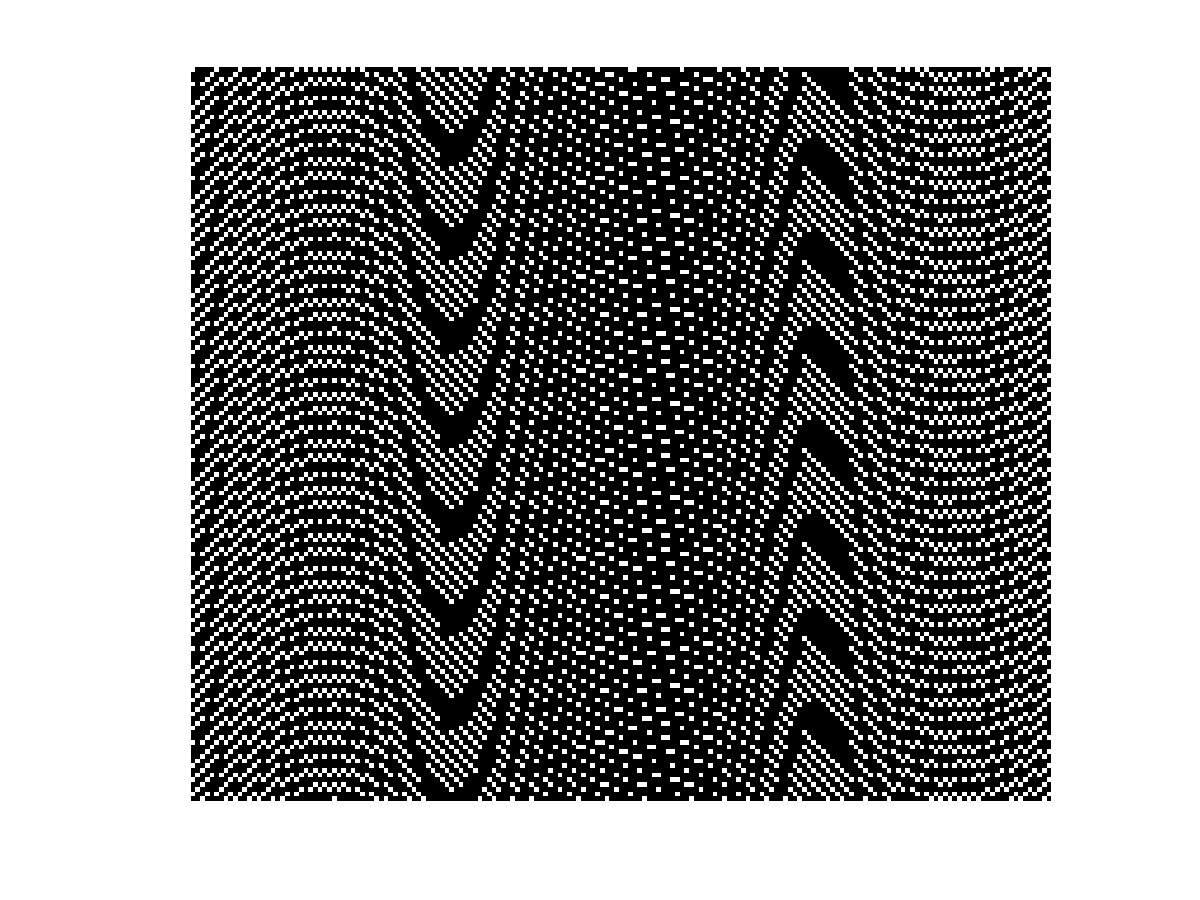
\includegraphics[width=0.35\textwidth]{sample_9} & 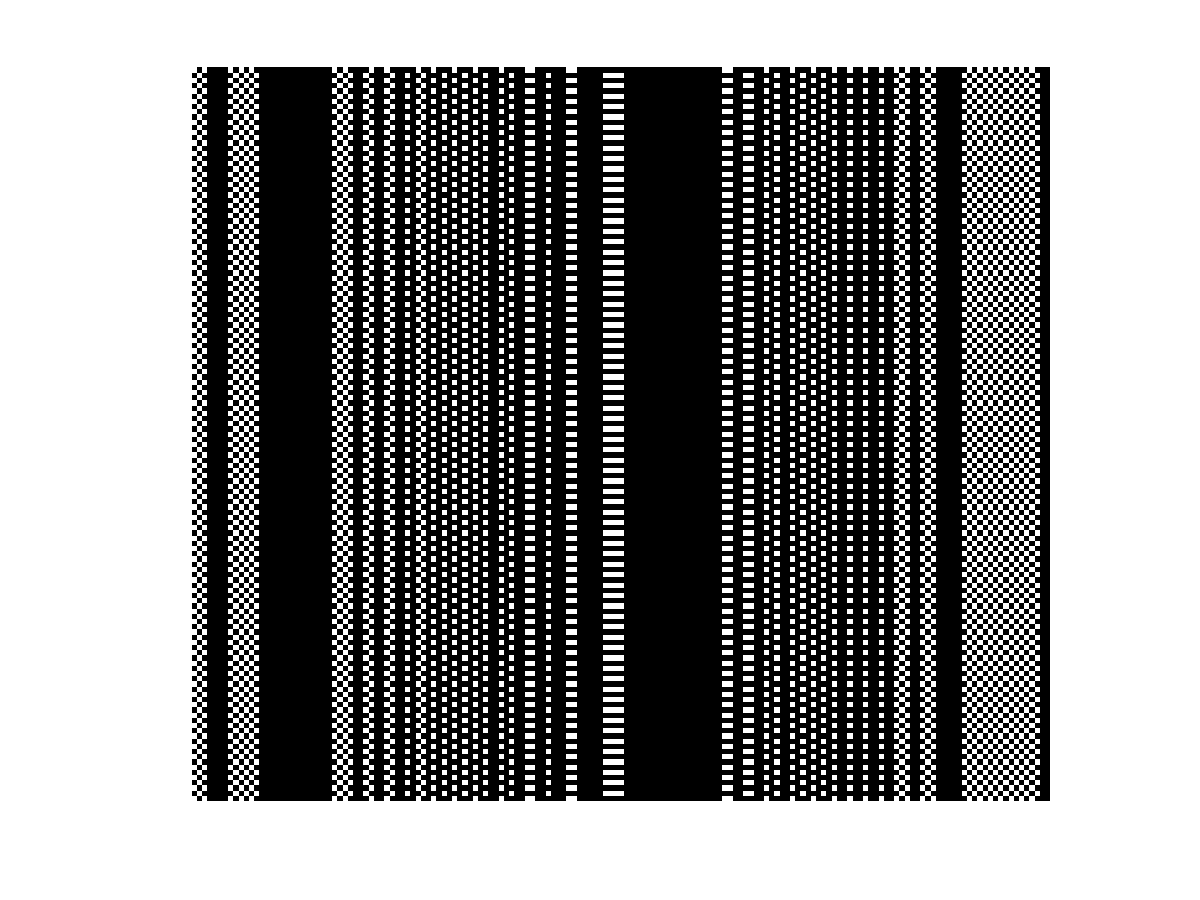
\includegraphics[width=0.35\textwidth]{sample_10}
                    \end{tabular}
                    \caption{Rezultati otipkavanja s faktorima od 1 do 10}
                    \label{fig:sampling}
                \end{figure}
                \item 
                    Kod viših faktora otipkavanja gube se više frekvencije na slici i gube se informacije. Vidi sliku \ref{fig:sampling}
            \end{enumerate}
        \section{Pikselizacija}
            \begin{enumerate}
                \item
                    \begin{minipage}{\linewidth}
                        \centering
                        
\includegraphics[width=0.75\textwidth]{baltazar}
                        \captionof{figure}{Slika cenzurirana pikselizacijom jedne regije.}
                    \end{minipage}
                \item
                    Parametar {\it nearest} određuje metodu interpolacije kad se dimenzije slike povećavaju.
                    {\it Nearest} metoda samo pridružuje vrijednost najbližeg piksela.
            \end{enumerate}
        \section{Alias-efekt}
            \begin{enumerate}
                \begin{figure}[ht]
                    \centering
                    \begin{tabular}{cc}
                        
\includegraphics[width=0.35\textwidth]{sampleL_1} & 
\includegraphics[width=0.35\textwidth]{sampleL_2} \\
                        
\includegraphics[width=0.35\textwidth]{sampleL_3} & 
\includegraphics[width=0.35\textwidth]{sampleL_4} \\
                        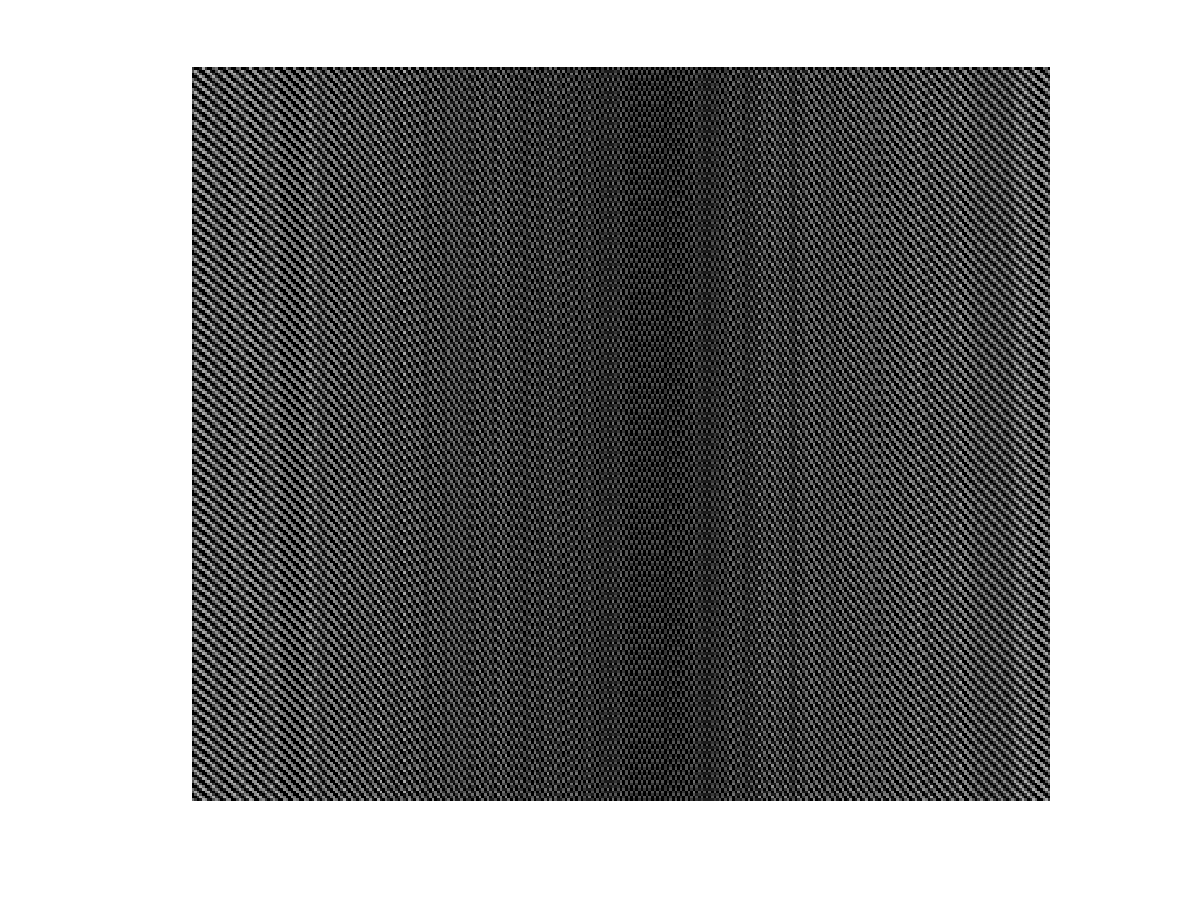
\includegraphics[width=0.35\textwidth]{sampleL_5} & 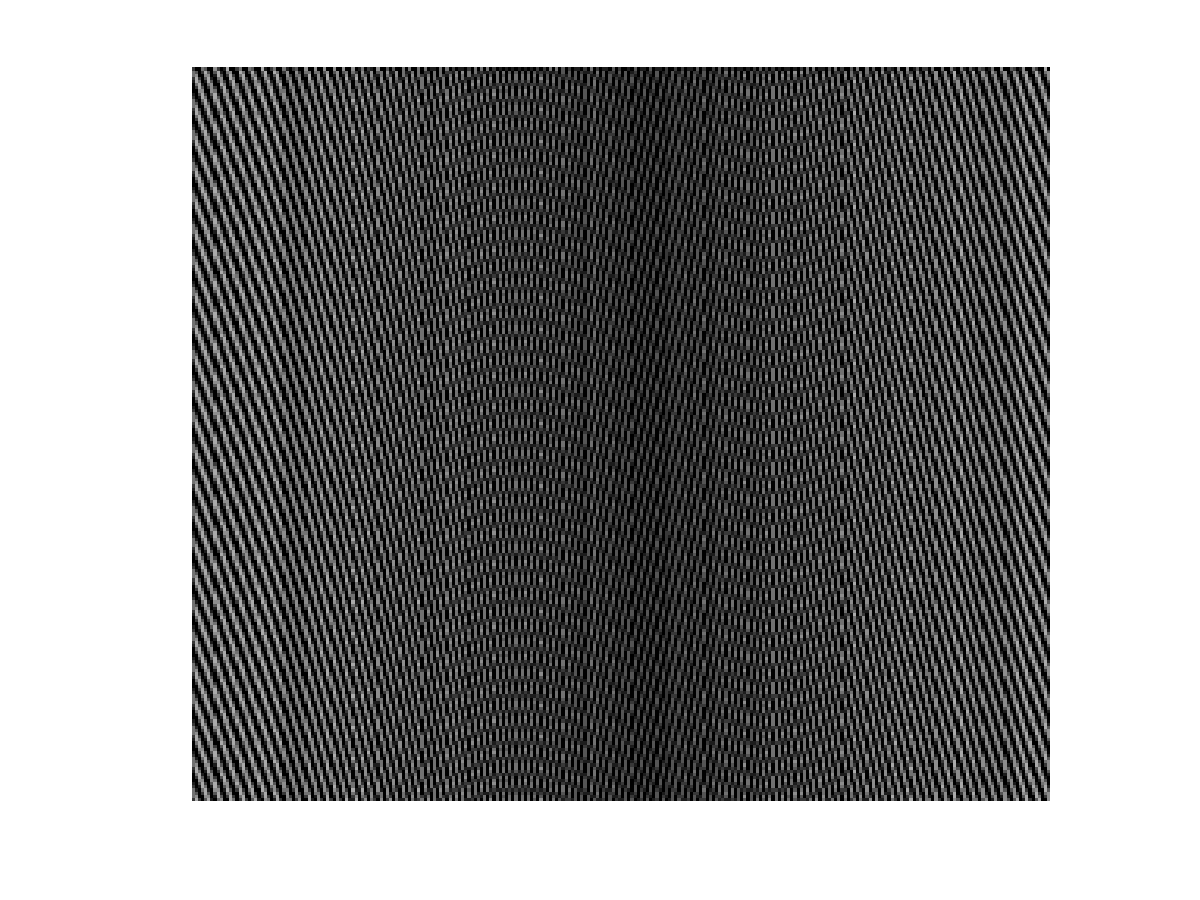
\includegraphics[width=0.35\textwidth]{sampleL_6} \\
                        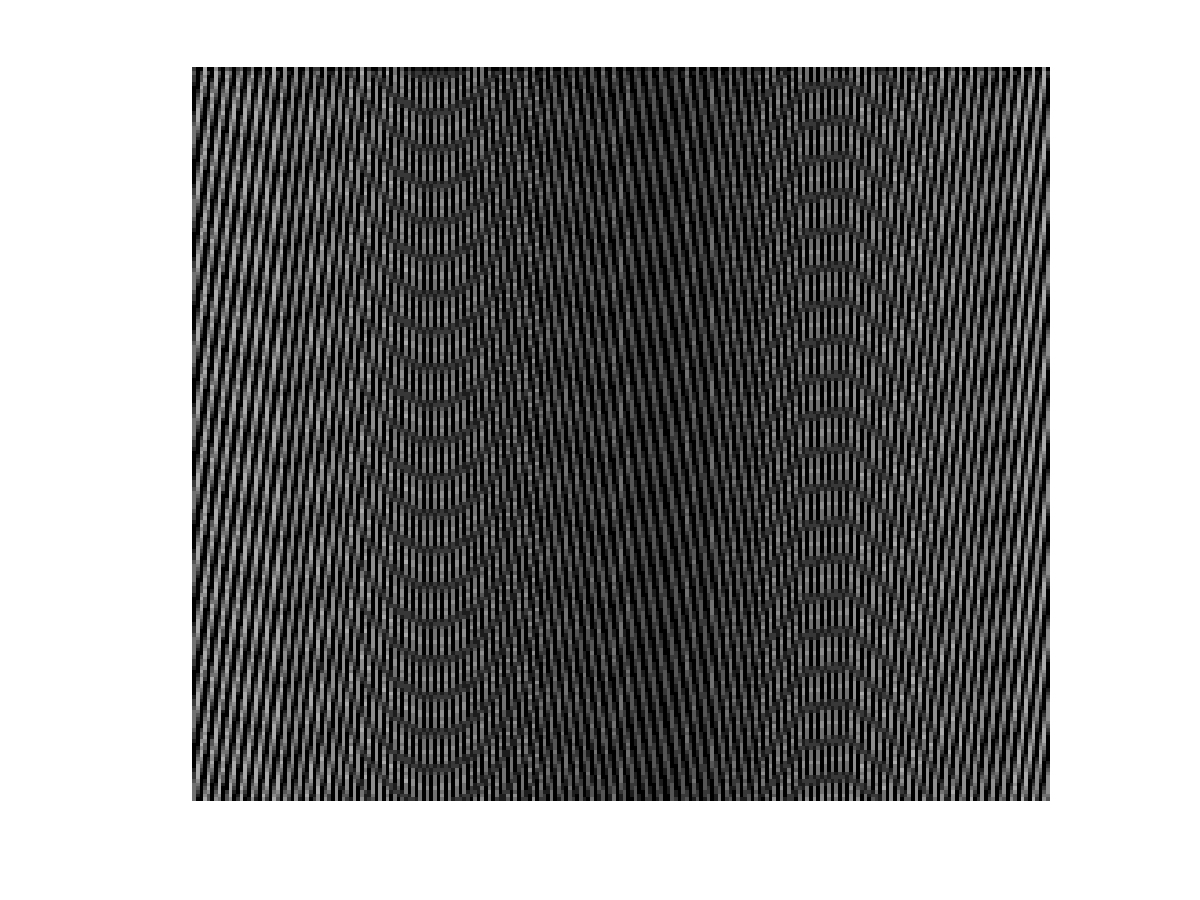
\includegraphics[width=0.35\textwidth]{sampleL_7} & 
\includegraphics[width=0.35\textwidth]{sampleL_8} \\
                        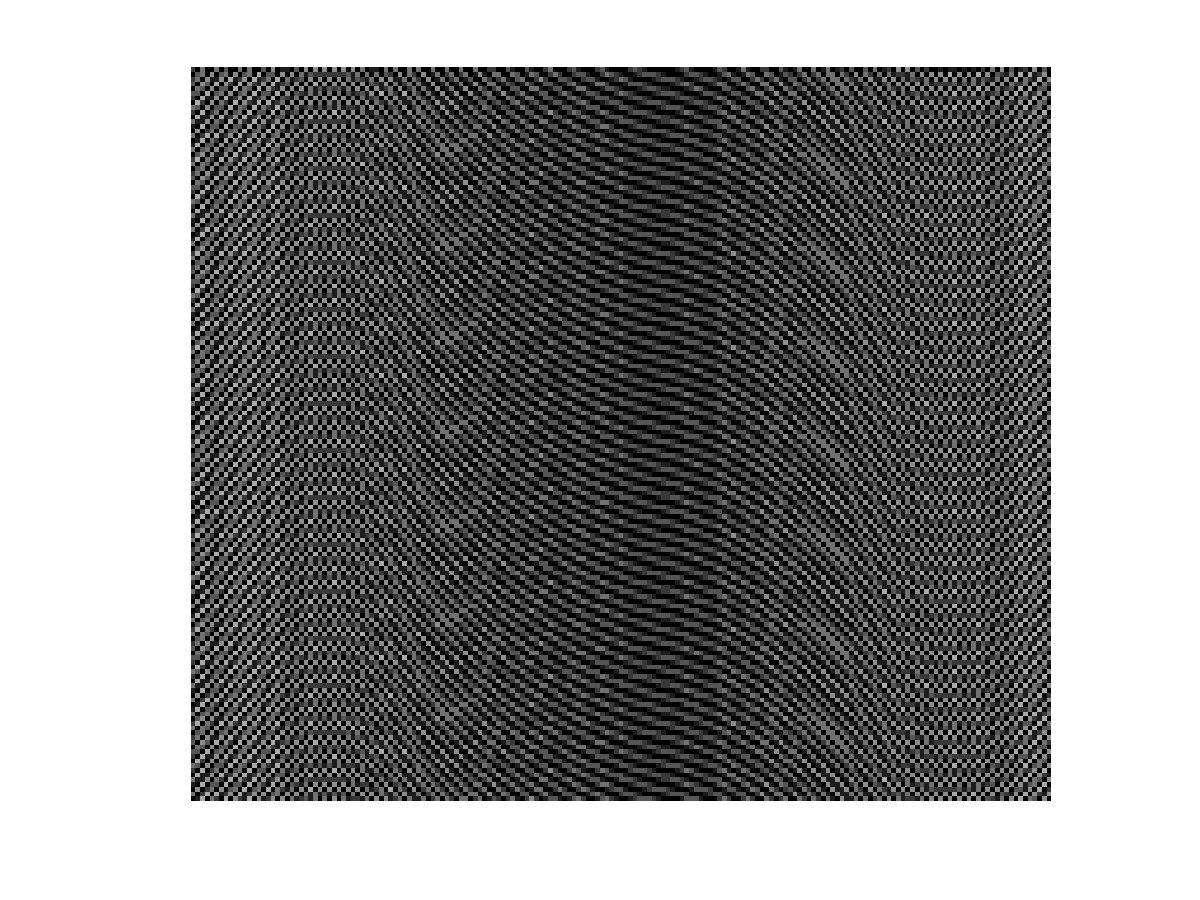
\includegraphics[width=0.35\textwidth]{sampleL_9} & 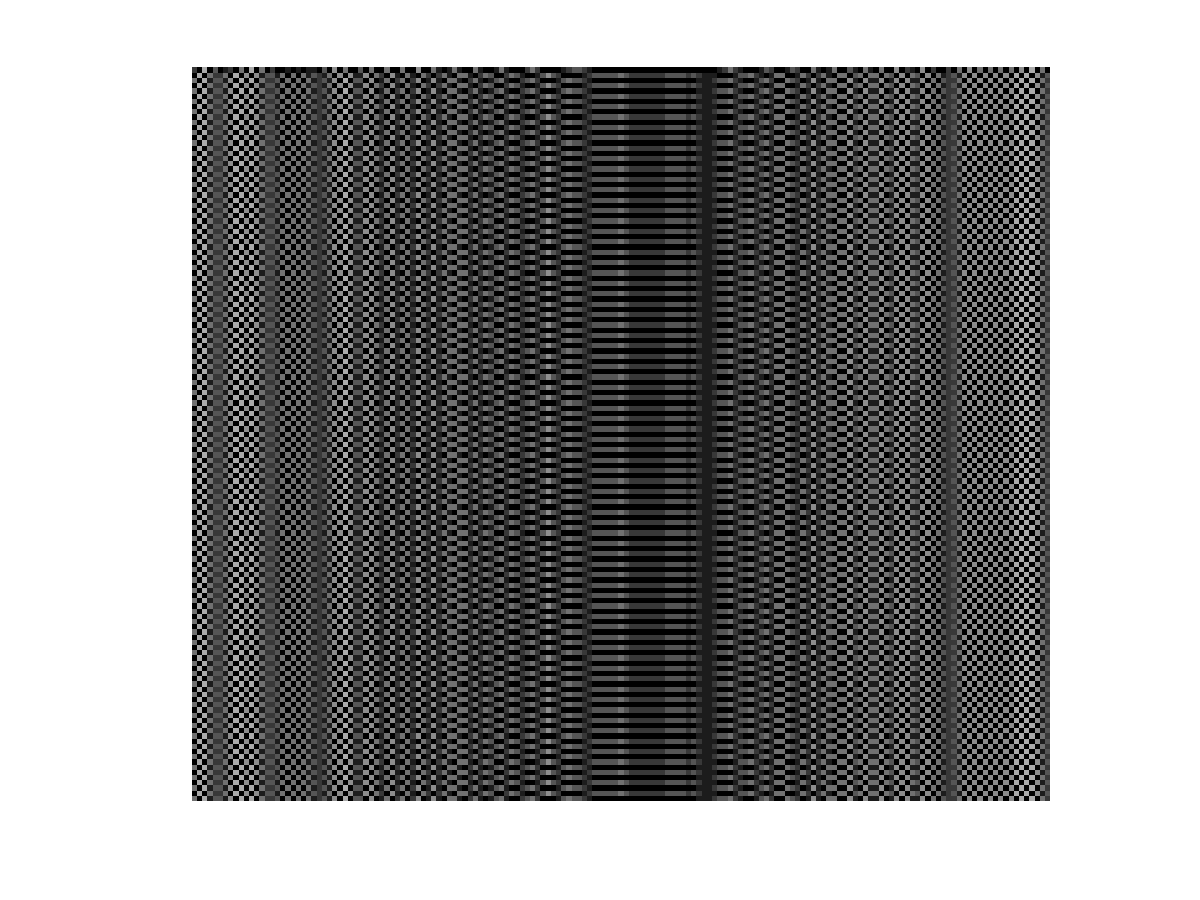
\includegraphics[width=0.35\textwidth]{sampleL_10}
                    \end{tabular}
                    \caption{Rezultati otipkavanja s faktorima od 1 do 10 nakon zamućenja slike}
                    \label{fig:sampling2}
                \end{figure}
                \begin{figure}
                    \centering
                    \begin{tabular}{cc}
                        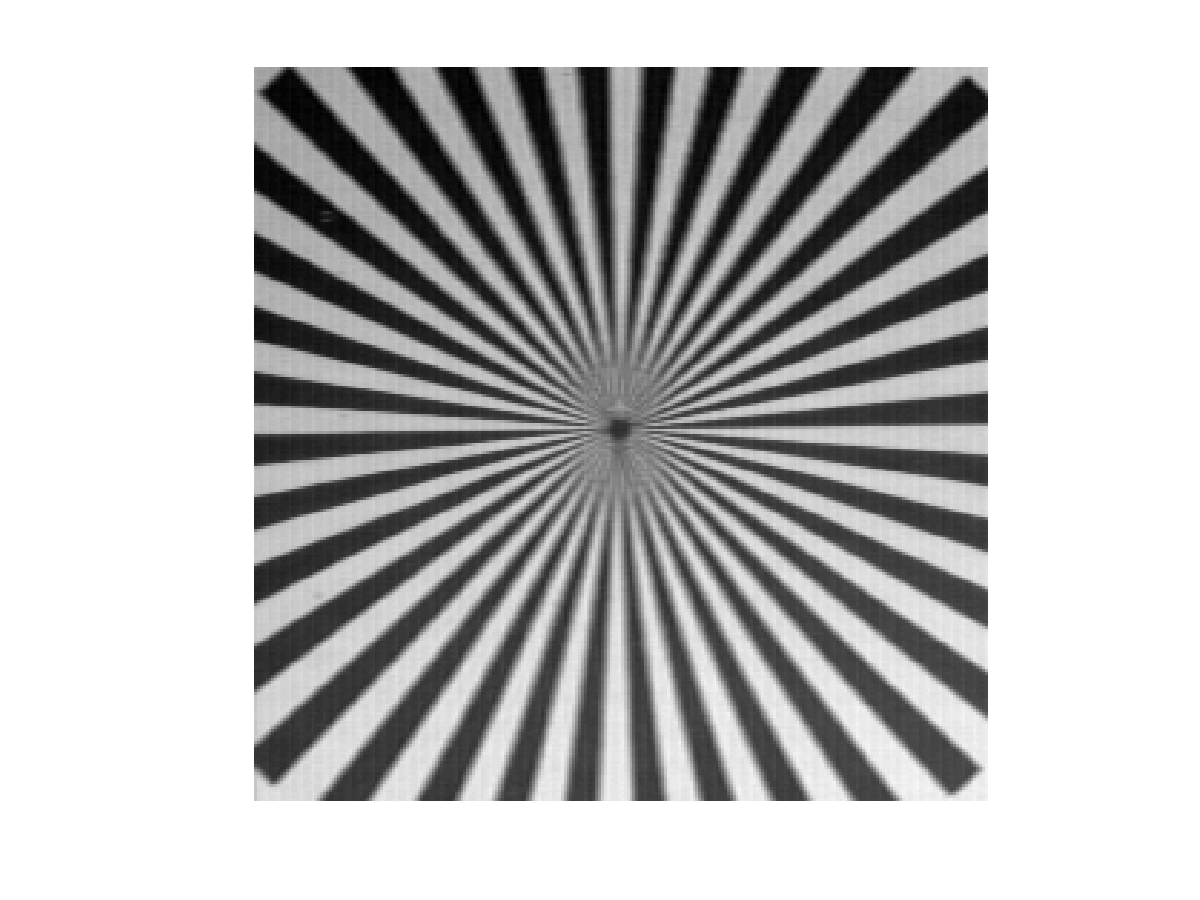
\includegraphics[width=0.35\textwidth]{testpat1} & 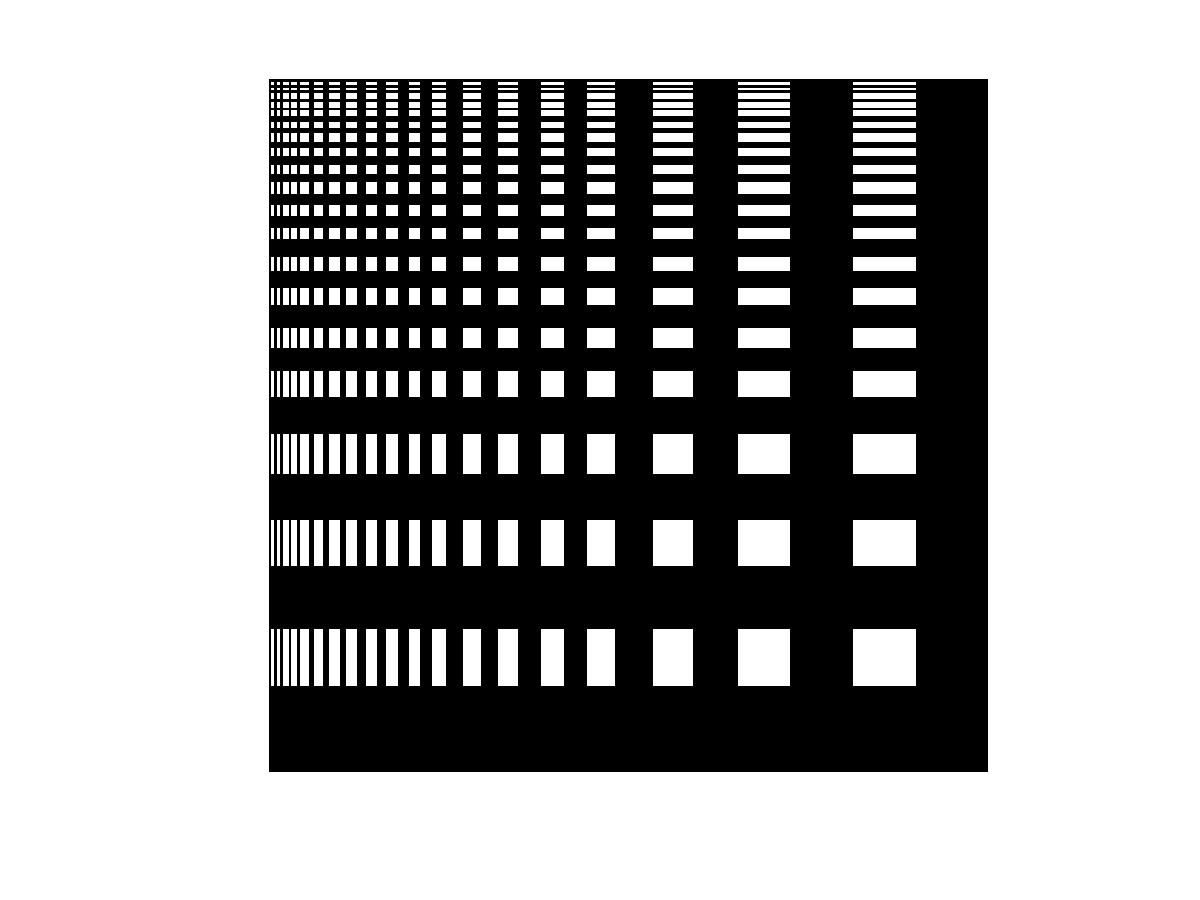
\includegraphics[width=0.35\textwidth]{testpat2} \\
                        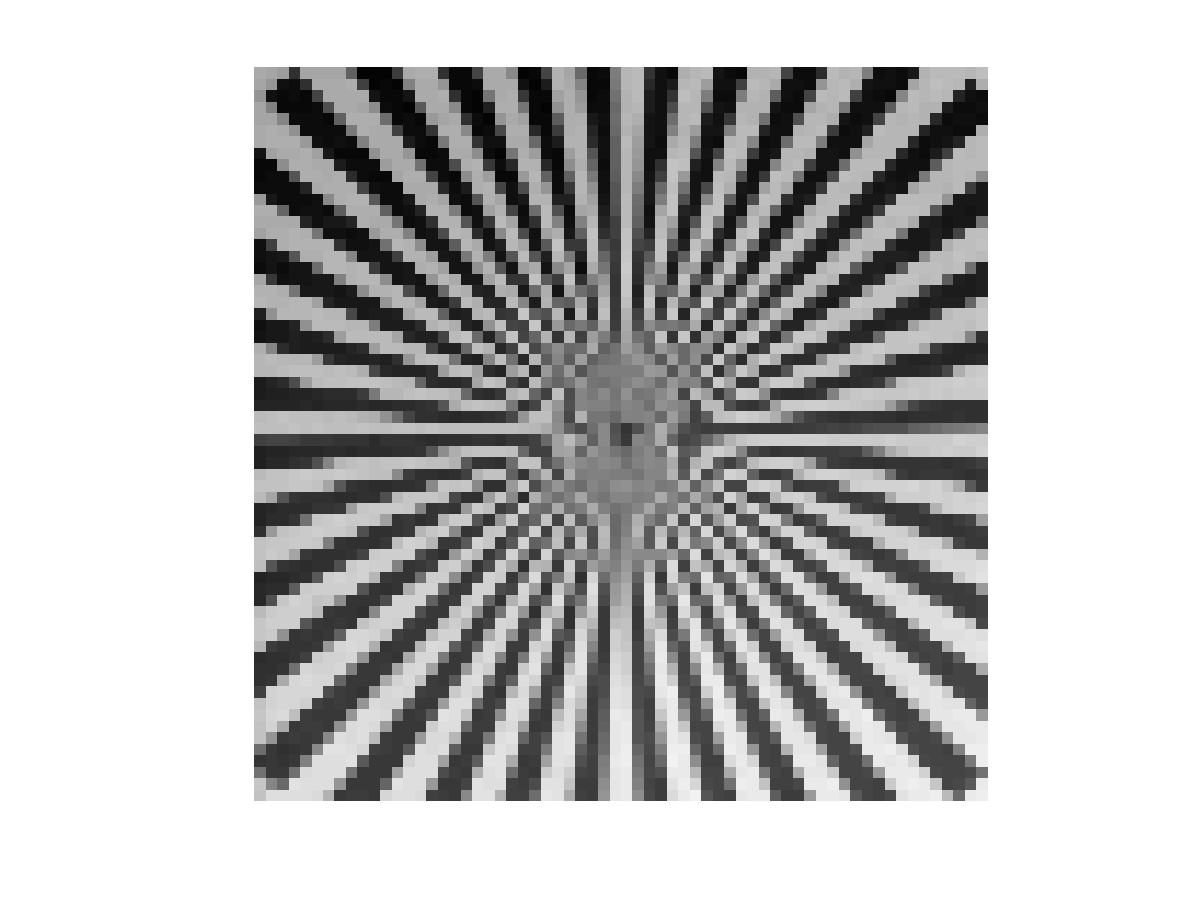
\includegraphics[width=0.35\textwidth]{testpat1S} & 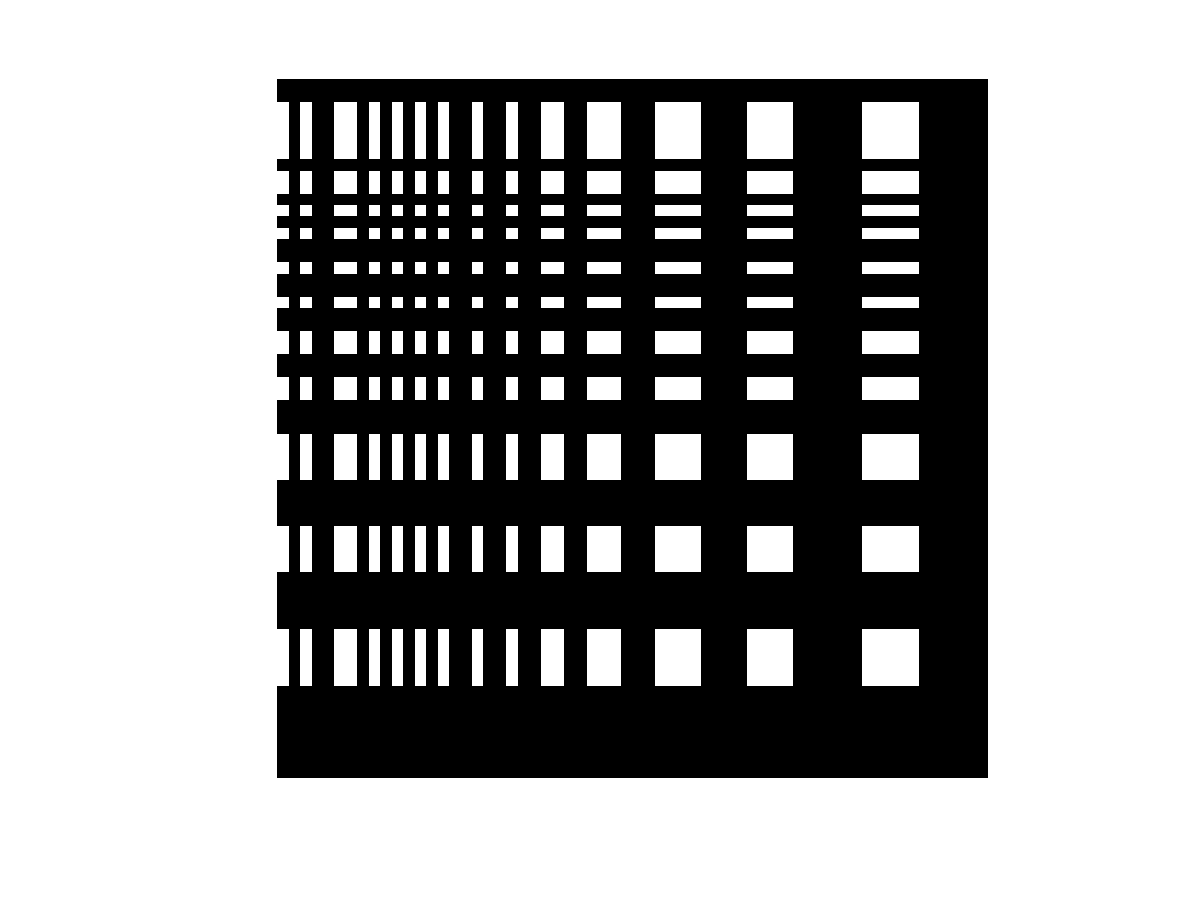
\includegraphics[width=0.35\textwidth]{testpat2S}
                    \end{tabular}
                    \caption{Rezultati otipkavanja slika {\it testpat1.tif} i {\it testpat2.tif}. Informacije o višim frekvencijama su izgubljene otipkavanjem.}    
                    \label{fig:sampling3}
                \end{figure}
                \begin{figure}
                    \centering
                    \begin{tabular}{cc}
                        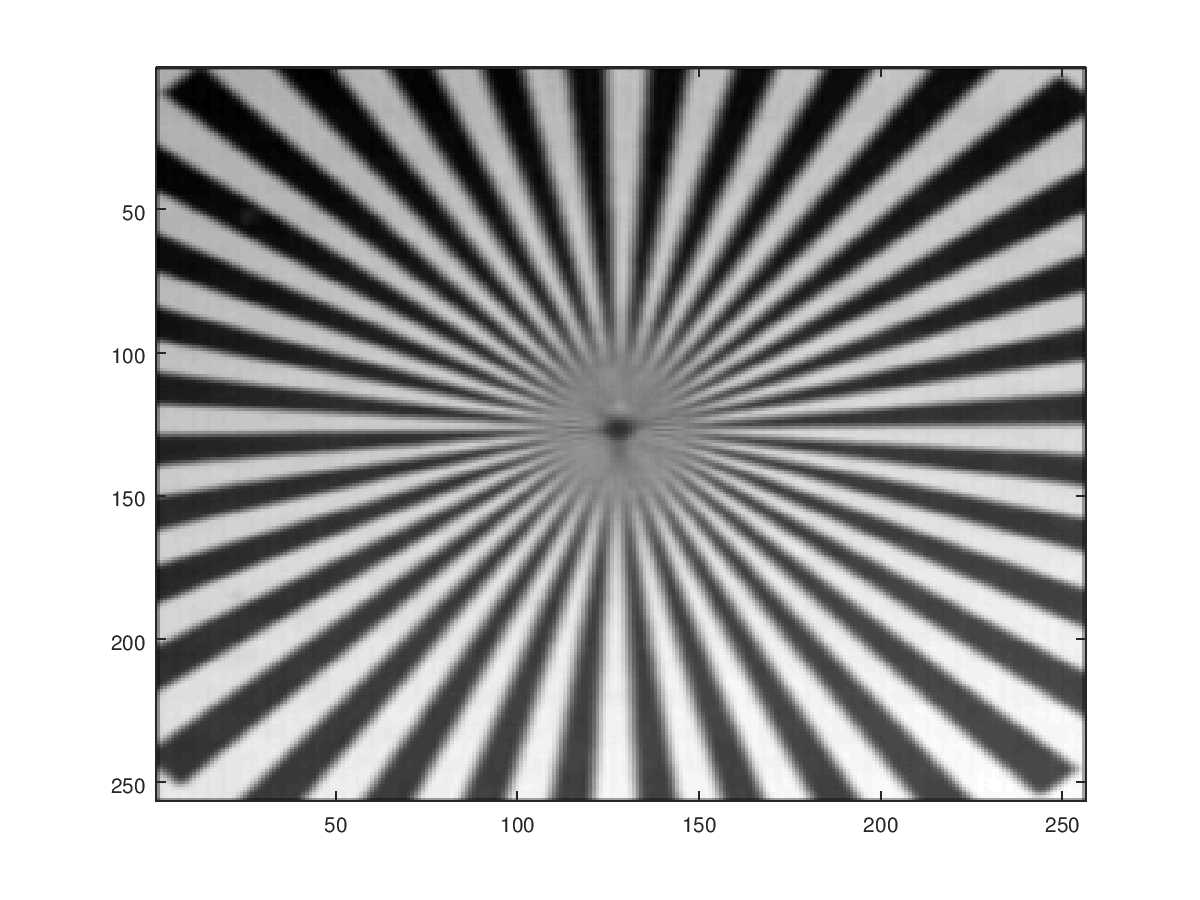
\includegraphics[width=0.35\textwidth]{testpat1L} & 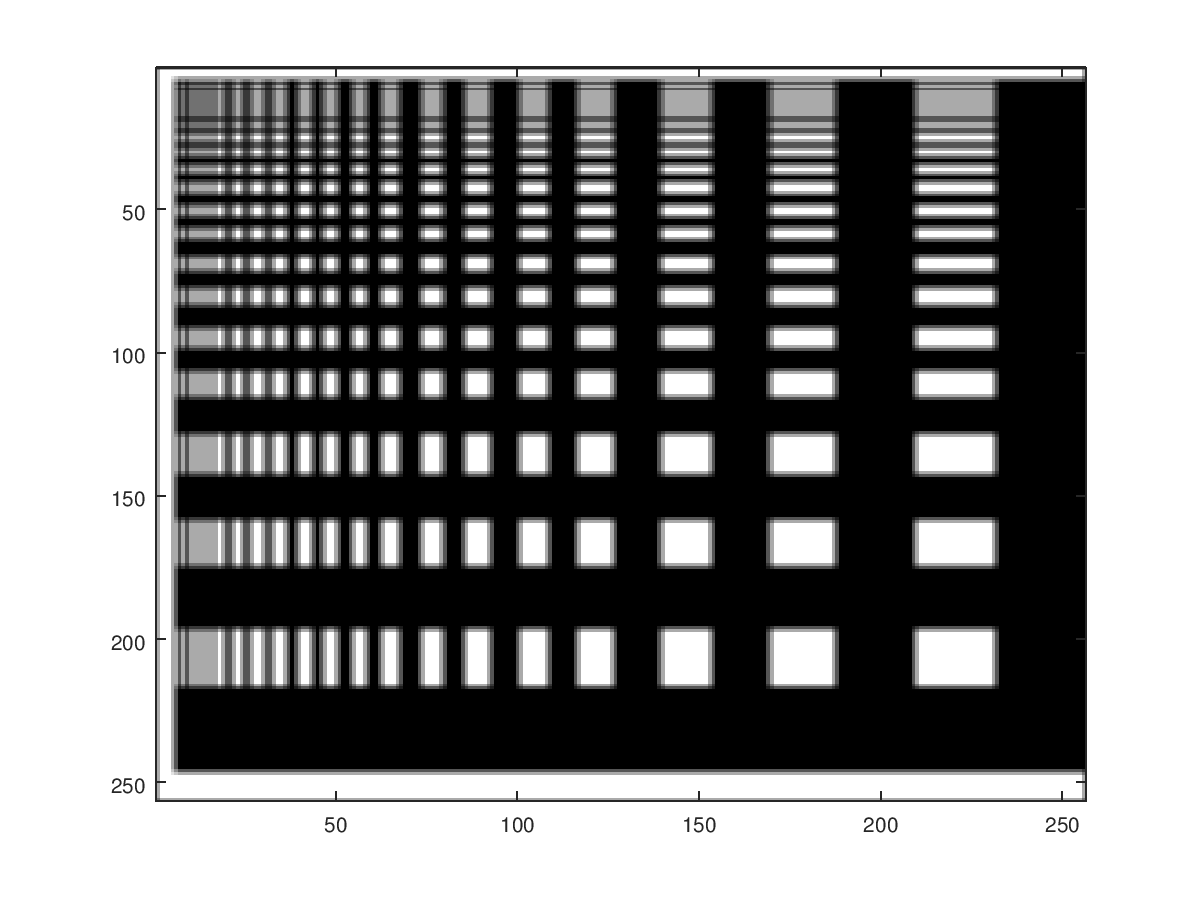
\includegraphics[width=0.35\textwidth]{testpat2L} \\
                        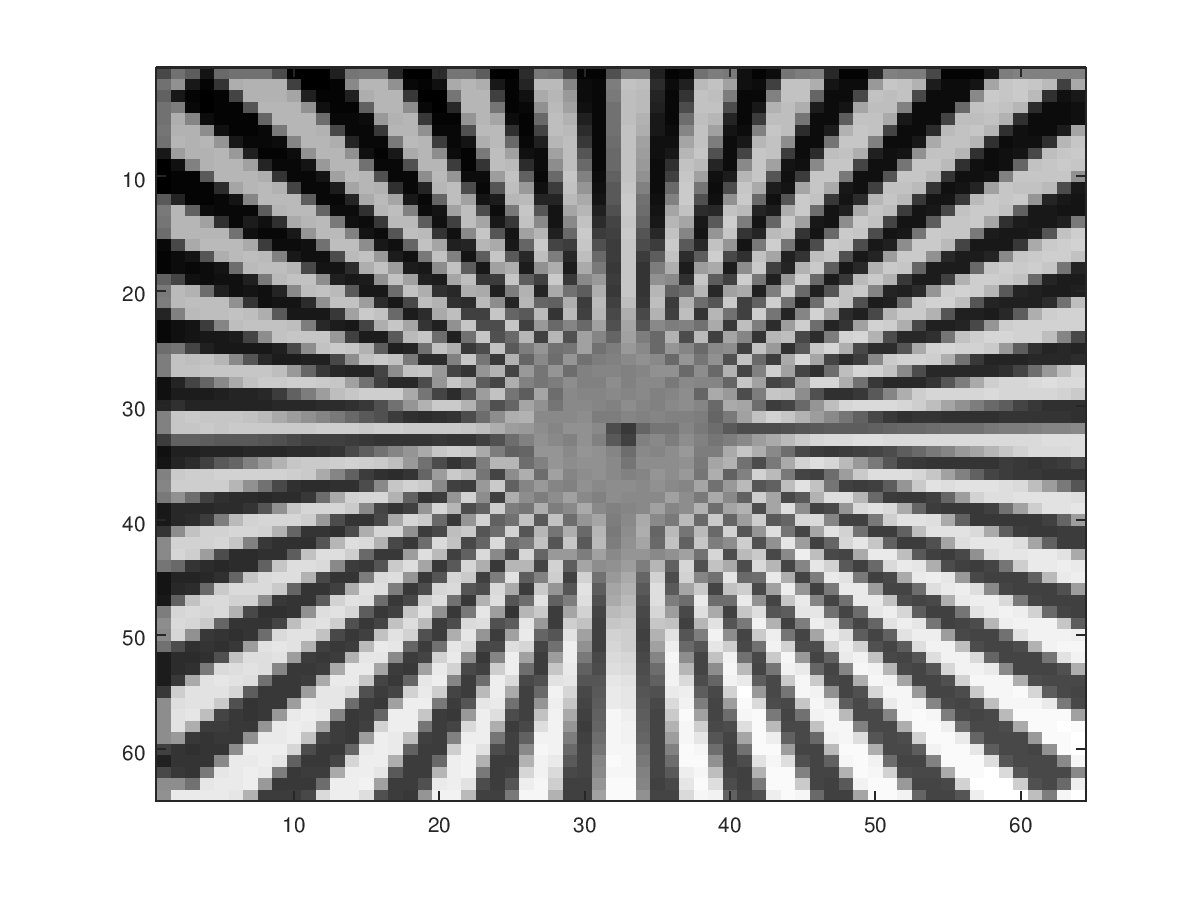
\includegraphics[width=0.35\textwidth]{testpat1LS} & 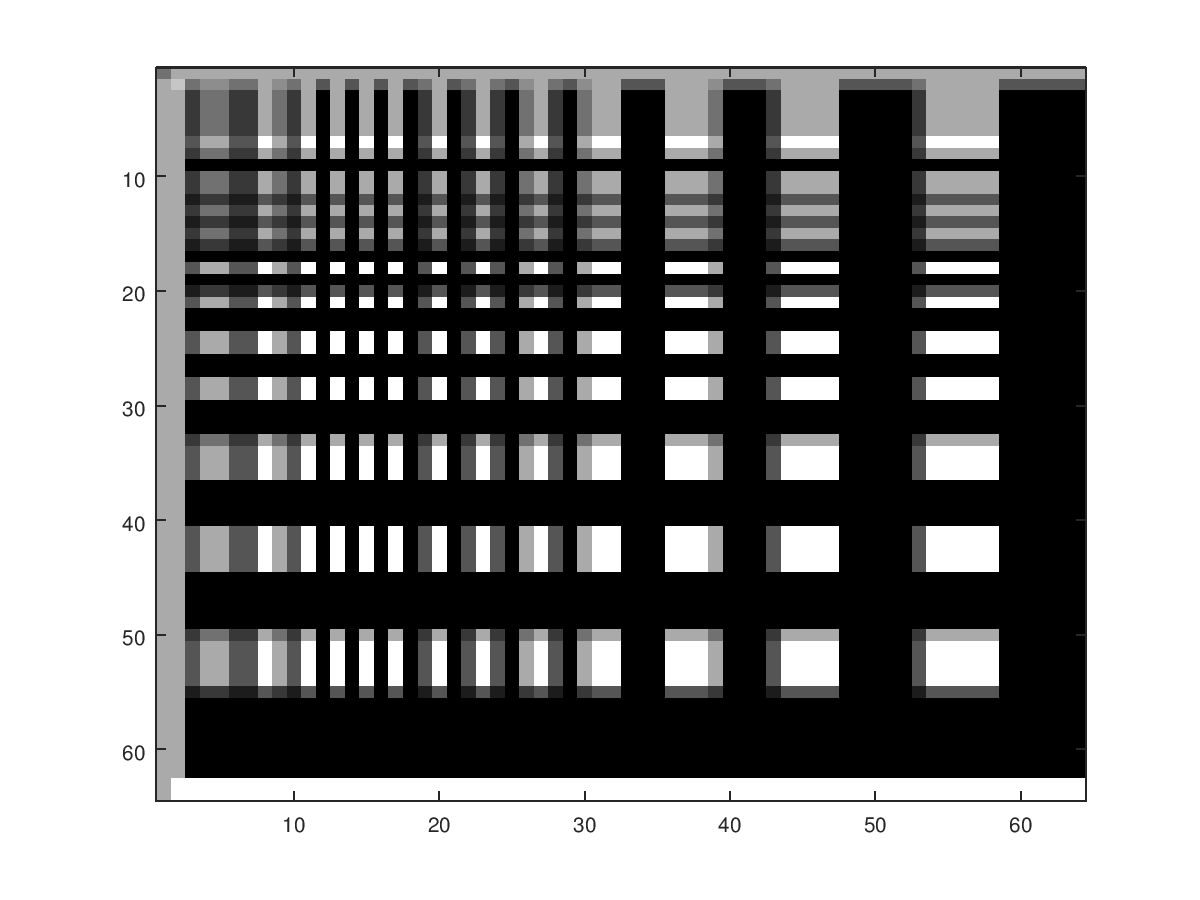
\includegraphics[width=0.35\textwidth]{testpat2LS}
                    \end{tabular}
                    \caption{Rezultati otipkavanja slika {\it testpat1.tif} i {\it testpat2.tif} nakon zamućenja.}    
                    \label{fig:sampling4}
                \end{figure}
                \begin{figure}
                    \centering
                    \begin{tabular}{cc}
                        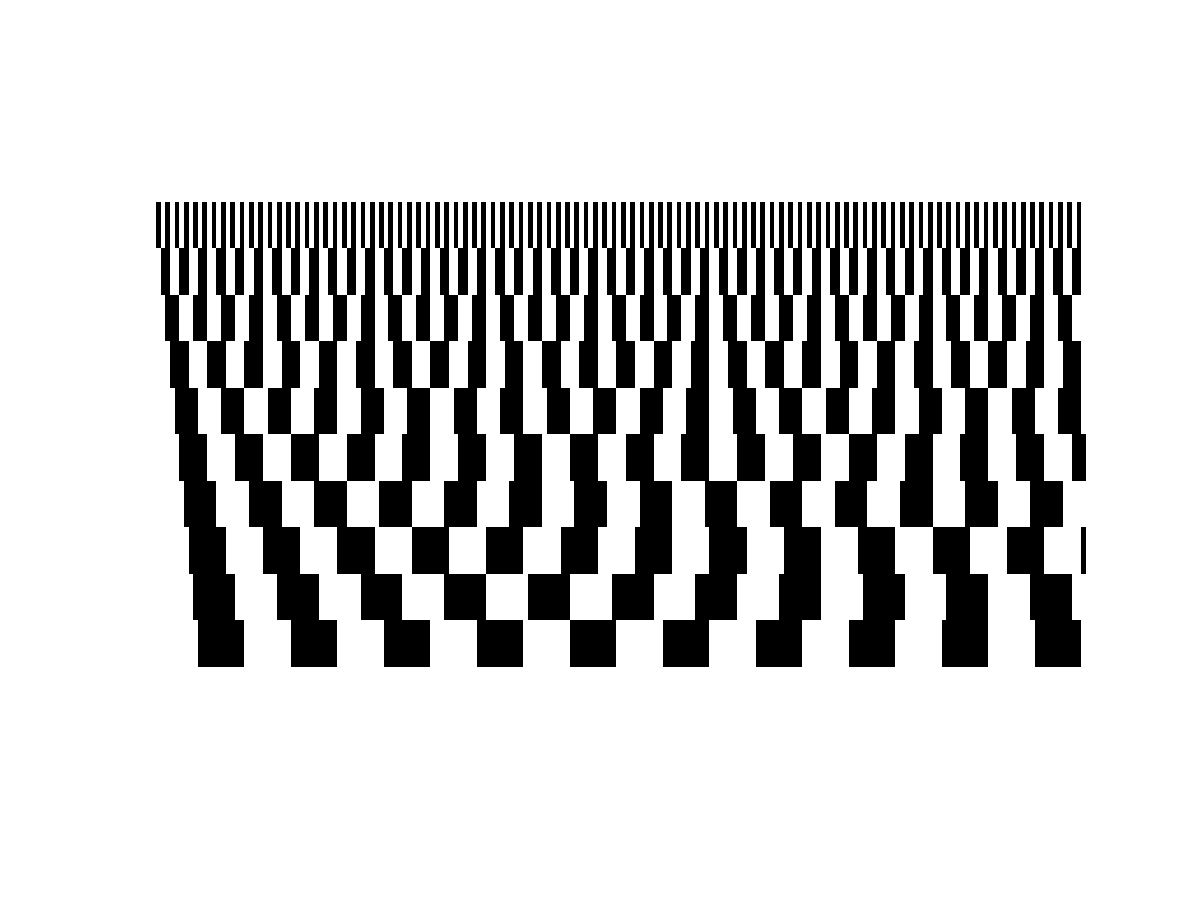
\includegraphics[width=0.35\textwidth]{uzorakS1} & 
\includegraphics[width=0.35\textwidth]{uzorakS2} \\
                        (a) & (b)
                    \end{tabular}
                    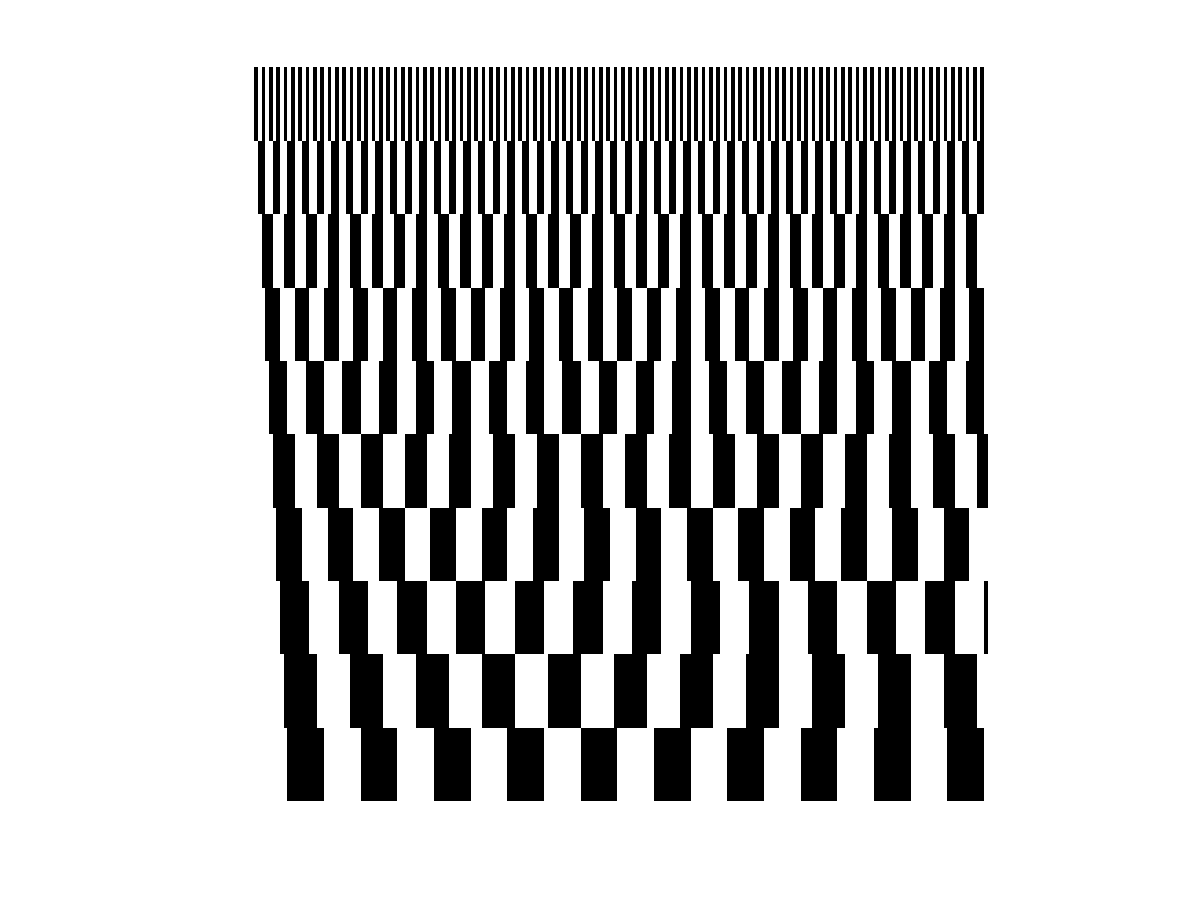
\includegraphics[width=0.35\textwidth]{uzorak} \\
                    (c)
                    \caption{Podtipkavanjem slike (c) po osi X (b) je izgubljeno više informacija jer je frekvencija viša.}    
                    \label{fig:sampling5}
                \end{figure}
                \begin{figure}
                    \centering
                    \begin{tabular}{cc}
                        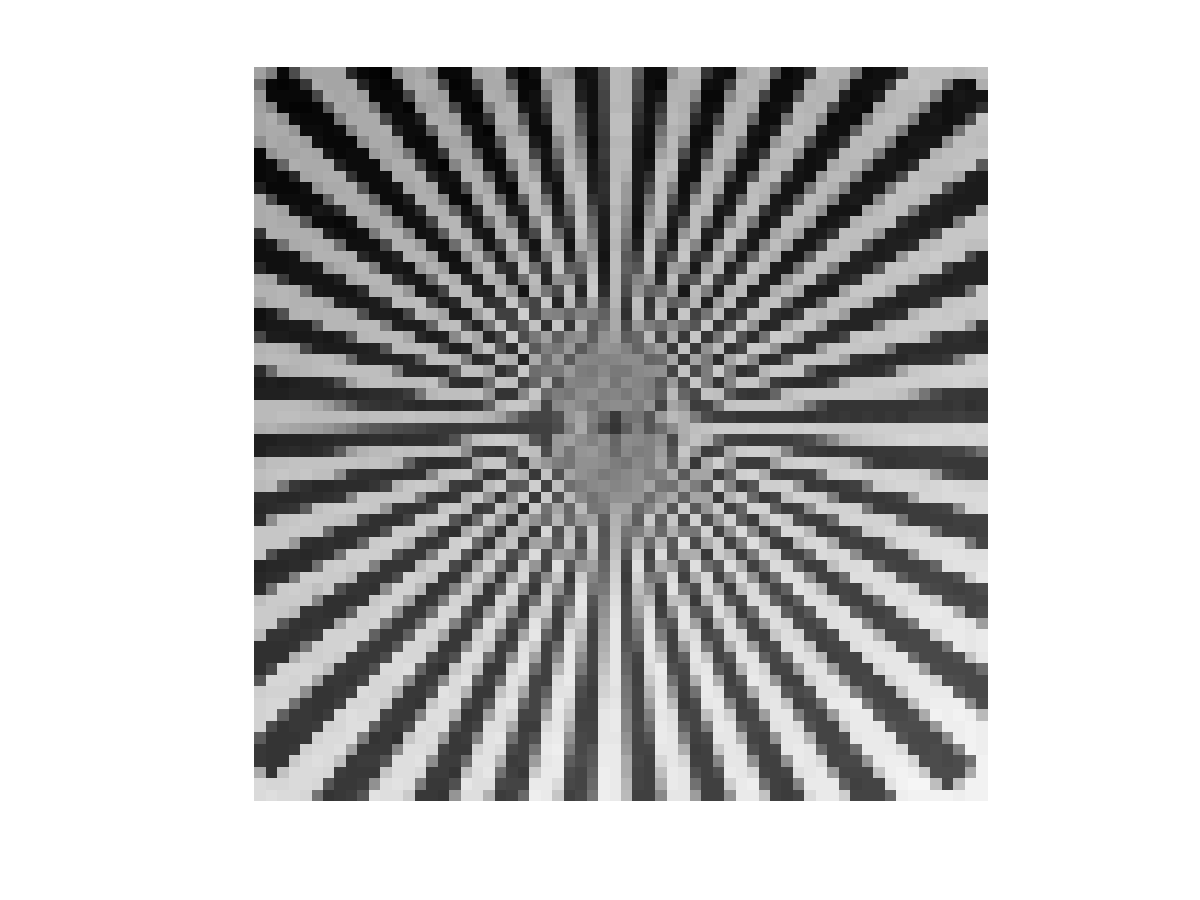
\includegraphics[width=0.35\textwidth]{testpat1small} & 
\includegraphics[width=0.35\textwidth]{uzoraksmall}\\
                        (a) & (b)
                    \end{tabular}
                    \caption{Rezultati se ne razlikuju previše jer je smanjenje slike 4 puta sa {\it nearest} interpolacijom samo aliasing sa faktorom 4. Ako koristimo neku bolju metodu interpolacije možemo izbjeći predfiltriranje.}    
                    \label{fig:sampling6}
                \end{figure}
                \begin{figure}
                    \centering
                    \begin{tabular}{cc}
                        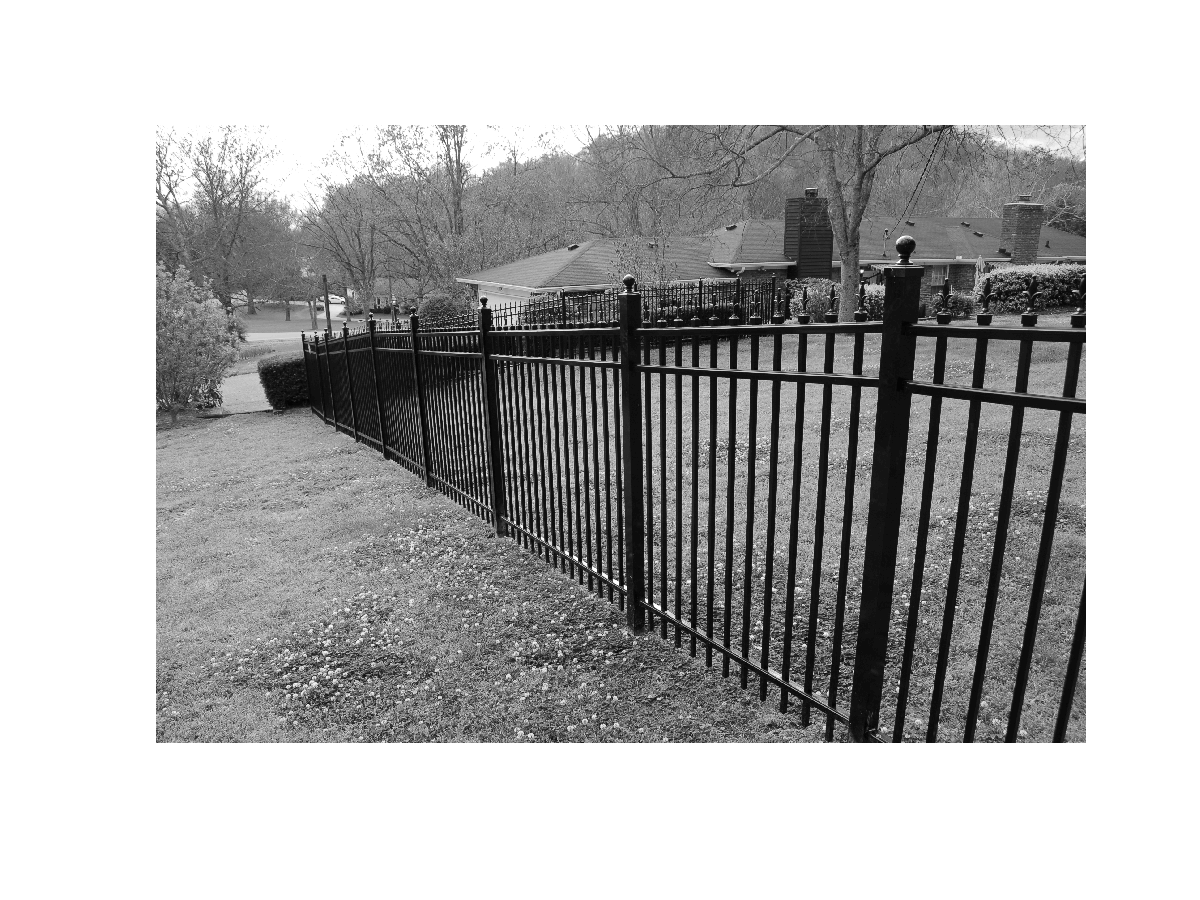
\includegraphics[width=0.35\textwidth]{fence} & \includegraphics[width=0.35\textwidth]{fenceAlias}\\
                        (a) & (b)
                    \end{tabular}
                    \caption{Primjer alias efekta na slici prirodne scene.}    
                    \label{fig:sampling7}
                \end{figure}
                \item 
                    Rezultat podotipkavanja nakon zamućenja je bolji nego prije jer se zamućenjem gube visoke frekvencije, te jer se informacije 
                    šire na susjedne piksele, manji je gubitak informacija. Slika \ref{fig:sampling2}               
                \item
                    Vidi slike \ref{fig:sampling2}, \ref{fig:sampling3}, \ref{fig:sampling4}, \ref{fig:sampling5}, \ref{fig:sampling6}, \ref{fig:sampling7}
            \end{enumerate}
        \section{Moarški efekt}
            \begin{figure}
                \centering
                \begin{tabular}{cc}
                    \includegraphics[width=0.35\textwidth]{ab2} & \includegraphics[width=0.35\textwidth]{ab21} \\
                    (a) & (b) \\
                    \includegraphics[width=0.35\textwidth]{ab22} & \includegraphics[width=0.35\textwidth]{ab23} \\
                    (c) & (d)
                \end{tabular}
                \caption{Uzorkovanjem odgovarajućim faktorom po osi y mogu se dobiti uzorci koji se ponavljaju u originalnoj slici.}    
                \label{fig:moire}
            \end{figure}
            \begin{enumerate}
                \item Vidi sliku \ref{fig:moire}
            \end{enumerate}
    \end{document}  